\documentclass[12pt,journal,compsoc, onecolumn]{IEEEtran}

\usepackage[pdftex]{graphicx}   
\usepackage{cite}
\usepackage[utf8]{inputenc}
\usepackage[T1]{fontenc}
\usepackage{amsmath}
\usepackage{amsfonts}
\usepackage{amssymb}
\usepackage{hyperref}
\hypersetup{colorlinks=true, linkcolor=[rgb]{0,0,1}, citecolor=[rgb]{0,0,1}}
\usepackage{graphicx}
\usepackage{lmodern}
\usepackage{physics}
% \usepackage[left=1cm,right=1cm,top=2cm,bottom=1.5cm]{geometry}
\usepackage{siunitx}
\usepackage{fancyhdr}
\usepackage{enumerate}
\usepackage{mhchem}
\usepackage{mathrsfs}
\usepackage{mathtools}
\usepackage{graphicx}
\usepackage{tabularx}
\usepackage{float}
\usepackage{xcolor}
\usepackage{mdframed}
\usepackage{csquotes}
\usepackage{trfsigns}
\usepackage{capt-of}
\usepackage{booktabs}
\usepackage{comment}
\usepackage{amsmath}
\usepackage{algorithm}
\usepackage{amsthm}
\usepackage[noend]{algpseudocode}
\usepackage[
singlelinecheck=false % <-- important
]{caption}



\makeatletter
\def\BState{\State\hskip-\ALG@thistlm}
\makeatother

\usepackage{fixltx2e}
\usepackage{xcolor}
\def\SPSB#1#2{\rlap{\textsuperscript{\textcolor{red}{#1}}}\SB{#2}}
\def\SP#1{\textsuperscript{\textcolor{red}{#1}}}
\def\SB#1{\textsubscript{\textcolor{blue}{#1}}}

\newcommand{\subparagraph}{}
\usepackage{titlesec}

\setcounter{secnumdepth}{4}

\titleformat{\paragraph}
{\normalfont\normalsize\bfseries}{\theparagraph}{1em}{}
\titlespacing*{\paragraph}
{0pt}{3.25ex plus 1ex minus .2ex}{1.5ex plus .2ex}

\mdfdefinestyle{exercise}{
	backgroundcolor=black!10,roundcorner=8pt,hidealllines=true,nobreak
}



\newtheorem{theorem}{Theorem}[section]
\newtheorem{corollary}{corollary}[theorem]
\newtheorem{lemma}[theorem]{Lemma}
\newtheorem{definition}[theorem]{Definition}
\newtheorem{proposition}[theorem]{Proposition}
\newtheorem{remark}[theorem]{Remark}
\newtheorem{example}[theorem]{Example}






\begin{document}

\title{Spurious Quasi-Resonances for Stabilized BIE-Volume Formulations for the Helmholtz Transmission Problem}

\author{Frederic Jørgensen. \textit{\today}}




\IEEEtitleabstractindextext{%
\begin{abstract}
\noindent 
A particular \textit{regularised variational formulation} of the Helmholtz transmission problem is studied on a two-dimensional disk for varying frequencies. In particular, the operator norm of its associated inverse operator is investigated.
In scenarios where the inner refractive index is bigger than the outer one, the operator norm associated with the considered formulation resonates and grows as a function of the wave number. The solution operator did not expose this resonance and growth behavior. This behavior, studied in previous research for other operators, is called \textit{spurious quasi-resonances}. The occurring resonances, however, were much weaker in the formulation considered here than in others. The origin of these resonances  is explained.
\end{abstract}}



\maketitle

\IEEEdisplaynontitleabstractindextext
\IEEEpeerreviewmaketitle



\section{Introduction}
\label{section:introduction}
\IEEEPARstart{L}{et} \(\Omega^- \subset \mathbb{R}^d, d > 0\) be a bounded Lipschitz domain and 
define \(\Omega^{+}:=\mathbb{R}^{d} \backslash \overline{\Omega^{-}}\), 
\(\Gamma := \partial \Omega^-\).
For any function $f$ on $\mathbb{R}^d$ define $f^\pm :=f|_{\Omega^{\pm}}$. \\
Let \(H_{\text {loc }}^{1}\left(\Omega^{\pm}, \Delta\right):=\left\{v: \chi v \in H^{1}\left(\Omega^{\pm}\right), \Delta(\chi v) \in L^{2}\left(\Omega^{\pm}\right) \text{ for} \forall\chi \in C_{\text {comp }}^{\infty}\left(\mathbb{R}^{d}\right)\right\}\), as defined in \cite{hiptmair2021spurious}.
Consider the Neumann and Dirichlet trace operators 
\begin{align}
    \gamma_{D}^{\pm}: & H_{\mathrm{loc}}^{1}\left(\Omega^{\pm}\right) \rightarrow H^{\frac{1}{2}}(\Gamma), \left(\gamma_{D}^{\pm} f\right)({x}):=f({x}) \nonumber \\
    \gamma_{N}^{\pm}: & H_{\mathrm{loc}}^1\left(\Omega^{\pm}, \Delta\right) \rightarrow H^{-\frac{1}{2}}(\Gamma), \left(\gamma_{N}^{\pm} f\right)({x}):=\operatorname{grad} f({x}) \cdot \mathbf{n}({x}) \nonumber
\end{align}
where \(H_{\mathrm{loc}}^{1}\left(\Omega^{\pm}\right)\),
\(H_{\mathrm{loc}}\left(\Delta, \Omega^{\pm}\right)\), 
\(H^{\frac{1}{2}}(\Gamma)\), and \(H^{-\frac{1}{2}}(\Gamma)\)
are defined in chapter 3 of  \cite{mclean2000strongly}.
Now, the Cauchy trace is \(\gamma_{C}^{\pm}: H_{\mathrm{loc}}^{1}\left(\Omega^{\pm}, \Delta\right) \rightarrow H^{1 / 2}(\Gamma) \times H^{-1 / 2}(\Gamma)\) with values given 
by \(\gamma_{C}^{\pm}:=\left(\gamma_{D}^{\pm}, \gamma_{N}^{\pm}\right)\). 
This concludes all required definitions to formulate the Helmholtz transmission problem.

\begin{definition}[Helmholtz transmission problem]
For $\tilde \kappa, c_i, c_o > 0$ and \({f} = (f^1, f^2) \in H^{1 / 2}(\Gamma) \times H^{-1 / 2}(\Gamma)\) find \(U \in H_{\operatorname{loc}}^{1}\left(\mathbb{R}^{d} \backslash \Gamma\right)\) 
such that

\begin{align}
    \left(\Delta+\tilde\kappa^{2} c_{i}\right) U^{-} &=0  \quad \text { in } \Omega^{-}  \nonumber \\
    \left(\Delta+\tilde\kappa^{2} c_{o}\right) U^{+} &=0  \quad \text { in } \Omega^{+} \label{eq:helmholtz} \\
    \gamma_{C}^{+} U^{+} - \gamma_{C}^{-} U^{-} &=f \quad  \text { on } \Gamma. \nonumber 
\end{align}
Additionally, $u$ must satisfy the Sommerfeld radiation condition 
\(\lim\limits_{r \rightarrow \infty} r^{\frac{d-1}{2}}\left(\frac{\partial U}{\partial r}-i \sqrt{c_o} \tilde \kappa U\right)=0\) 
where $r$ refers to the radial spherical coordinate. 
\end{definition}  
\noindent
This problem is well-posed and the solution is unique as shown in Lemma 2.2 of \cite{moiola2019acoustic}.
Hiptmair et al. considered the \textit{single-trace formulations} (STF) of this problem  \cite{hiptmair2021spurious}. 
This is a reformulation of this problem in terms of \textit{boundary integral equations} (BIEs). 
When investigating the case $c_i < c_o$ they found that the involved  \textit{boundary integral operators} (BIOs) as a
 function of $\tilde \kappa$ exposed a nonphysical resonance behavior. 
More specifically, they found the operator norm of the inverse STF BIOs to have resonances (called \textit{spurious quasi-resonances})
that the norm of the solution operator did not.
Formally, Hiptmair et al. defined the solution operator as follows \cite{hiptmair2021spurious}.
\begin{definition}
    \label{def:solution_operator}
    Given positive real numbers \(k, c_{i}\), and \(c_{o}\), 
    $S: H^{\frac{1}{2}}(\Gamma) \times H^{-\frac{1}{2}}(\Gamma) \rightarrow  H^{\frac{1}{2}}(\Gamma) \times H^{-\frac{1}{2}}(\Gamma)$ is the solution operator if 
     \(S\left(c_{i}, c_{o}\right) f:=\gamma_{C}^{-} u\)
    where \(u\) solves eq \ref{eq:helmholtz}.
\end{definition}
\noindent Hiptmair et al. removed these \textit{spurious quasi-resonances} 
using an augmented formulation of the BIEs.  P. Meury's doctoral thesis contained a \textit{regularized variational formulation} of the Helmholtz transmission problem \cite{meury2007stable}. 
The goal of this report is to investigate the occurrence of \textit{spurious quasi-resonance}
in this  {regularized variational formulation} of the Helmholtz transmission problem. 
For easier notation, let $\kappa = \tilde \kappa \sqrt{c_o}$ and $\tilde c := \frac{c_i}{c_o}$ on the following pages. Moreover, for the rest of the report
we consider the simple representational example $d = 2$ and $\Omega^- = B_1(0)$.
\\ Before reviewing this regularized variational formulation, we need to review a few concepts and introduce some notations.

\section{Definitions}
\label{section:definitions}
We review some basic definitions which are necessary in the coming sections.
The following definition was introduced in \cite{meury2007stable}.
\begin{definition}[Interior Dirichlet-to-Neumann map]
    The interior Interior Dirichlet-to-Neumann map  \(\operatorname{DtN}_{\kappa}^{-}: H^{\frac{1}{2}}(\Gamma) \times H^{-\frac{1}{2}}(\Gamma)\) is the operator that returns $\gamma_NU$ if $U$ solves the Dirichlet problem defined by a vector in $ H^{\frac{1}{2}}(\Gamma)$. 
\end{definition}
\noindent
Moreover, we will need the following BIOs defined in \cite{costabel1988boundary} \cite{meury2007stable}.
\begin{definition}
Let \(\left\{\gamma_{i} V\right\}_{\Gamma}:=\frac{1}{2}\left(\gamma_{i}^{+} V+\gamma_{i}^{-} V\right)\) for $i = D, N$. Moreover, introduce the single and double layer potential \(\Psi_{\mathrm{SL}}^{\kappa}(\vartheta)(\mathbf{x}):=\int_{\Gamma} G_{\kappa}(|\mathbf{x}-\mathbf{y}|) \vartheta(\mathbf{y}) \mathrm{d} S(\mathbf{y})\) and \(\Psi_{\mathrm{DL}}^{\kappa}(v)(\mathbf{x}):=\int_{\Gamma} \frac{\partial G_{\kappa}(|\mathbf{x}-\mathbf{y}|)}{\partial \mathbf{n}(\mathbf{y})} v(\mathbf{y}) \mathrm{d} S(\mathbf{y})\) with \(G_{\kappa}(z):=\frac{1}{4 \pi} \frac{\exp (i \kappa z)}{z}\). 
Then for $|s| < \frac{1}{2}$ we define four BIOs:
\begin{align} 
\mathrm{V}_{\kappa}: H^{s-\frac{1}{2}}(\Gamma) \rightarrow H^{s+\frac{1}{2}}(\Gamma), & \quad \mathrm{V}_{\kappa}:=\left\{\gamma_{D} \Psi_{\mathrm{SL}}^{\kappa}\right\}_{\Gamma} \nonumber\\ \mathrm{K}_{\kappa}: H^{s+\frac{1}{2}}(\Gamma) \rightarrow H^{s+\frac{1}{2}}(\Gamma), & \quad \mathrm{K}_{\kappa}:=\left\{\gamma_{D} \Psi_{\mathrm{DL}}^{\kappa}\right\}_{\Gamma} \nonumber \\ \mathrm{K}_{\kappa}^{\prime}: H^{s-\frac{1}{2}}(\Gamma) \rightarrow H^{s-\frac{1}{2}}(\Gamma), & \quad \mathrm{K}_{\kappa}^{\prime}:=\left\{\gamma_{N} \Psi_{\mathrm{SL}}^{\kappa}\right\}_{\Gamma} \nonumber\\ \mathrm{W}_{\kappa}: H^{s+\frac{1}{2}}(\Gamma) \rightarrow H^{s-\frac{1}{2}}(\Gamma), & \quad \mathrm{W}_{\kappa}:=-\left\{\gamma_{N} \Psi_{\mathrm{DL}}^{\kappa}\right\}_{\Gamma}. \nonumber
\end{align}
\end{definition} 
\noindent

\section{Regularized Variational Formulation}
\label{section:regularized_variational_formulation}

P. Meury provides a \textit{regularized variational formulation} of the Helmholtz tranmission problem as follows \cite{meury2007stable}.\footnote{The formulation provided here is equivalent to the case 
 $U_i = 0, f = 0, n(x) = c_i / c_o$ in section 3 of \cite{meury2007stable}.}
\begin{definition}[Regularized variational formulation]
    Find \(U \in H^{1}(\Omega), \theta \in H^{-1 / 2}(\Gamma)\) and \(p \in H^{1}(\Gamma)\) such that for all \(V \in H^{1}(\Omega), \varphi \in H^{-1 / 2}(\Gamma)\)
    and \(q \in H^{1}(\Gamma)\) there holds

    \begin{align}
        \mathrm{q}_{\kappa}(U, V)+\left(\mathrm{W}_{\kappa}\left(\gamma_{D}^{-} U\right), \gamma_{D}^{-} V\right)_{\Gamma}-\left((\frac{1}{2} \mathrm{ld}-\mathrm{K}_{\kappa}^{\prime})(\theta), \gamma_{D}^{-} V\right)_{\Gamma} &=g_1(V) \nonumber\\
        \left((\frac{1}{2} \mathrm{ld}-\mathrm{K}_{\kappa})\left(\gamma_{D}^{-} U\right), \varphi\right)_{\Gamma}+\left(\mathrm{fV}_{\kappa}(\theta), \varphi\right)_{\Gamma}+i \overline{\eta}(p, \varphi)_{\Gamma} &={g_2(\varphi)} \label{eq:variational_formulation}\\
        -\left(\mathrm{W}_{\kappa}\left(\gamma_{D}^{-} U\right), q\right)_{\Gamma}-\left((\mathrm{K}_{\kappa}^{\prime}+\frac{1}{2} \mathrm{Id})(\theta), q\right)_{\Gamma}+\mathrm{b}(p, q) &=g_3(q). \nonumber
    \end{align}

    where we have 
    $$
    \begin{aligned} 
        g_1(V) &:=-\left(f^2, \gamma_{D}^{-} V\right)_{\Gamma}-\left(\mathrm{W}_{\kappa}\left(f^1\right), \gamma_{D}^{-} V\right)_{\Gamma} \\ 
        g_2(\varphi) &:=\left(\left(\mathrm{K}_{\kappa}-\frac{1}{2} \mathrm{ld}\right)\left(f^1\right), \varphi\right)_{\Gamma} \\ 
        g_3(q) &:=\left(\mathrm{W}_{\kappa}\left(f^1\right), q\right)_{\Gamma} \\ 
        \mathrm{q}_{\kappa}(U, V)& :=\int_{\Omega} \operatorname{grad} U \cdot \operatorname{grad} \bar{V}-\kappa^{2} n({x}) U \bar{V} \mathrm{~d} {x} \\
        \mathrm{b}(p, q)& :=\left(\operatorname{grad}_{\Gamma} p, \operatorname{grad}_{\Gamma} q\right)_{\Gamma}+(p, q)_{\Gamma}.
    \end{aligned}
    $$

\end{definition}  \noindent
This formulation is derived from the Helmholtz transmission problem by partially integrating the Helmholtz equation, 
applying Green's first formula, coupling the resulting variational problem to 
the BIEs using Dirichlet-to-Neumann maps, and transforming the Cauchy trace \cite{meury2007stable}. 

%ToDO: mention eta stuff 


\section{Operator Formulation}
\label{section:operator_formulation}
The form of the variational problem in eq. \ref{eq:variational_formulation} can be rewritten in a simpler  operator formulation. 
We start by rewriting the expressions for $q_\kappa$ and $b$. 
\begin{lemma}\label{lem:reduced_q}
    Let $U, V \in H^{1}(\Omega^-)$ such that $U$ solves the Helmholtz equation. 
    Then $q_\kappa(U, V) = (\mathrm{DtN}_{ \kappa}^{-}\gamma_D^-U, V)_{\Gamma}$ with the
     Dirichlet-to-Neumann map $\mathrm{DtN}_{ \kappa}^{-}$.
\end{lemma}
\begin{proof}
    Greens first formula 
    \(\int\limits_{U}(\psi \operatorname{grad} \varphi+\operatorname{grad} \psi \cdot \operatorname{grad} \varphi) dx=
    \oint\limits_{\partial U} \psi \operatorname{grad} \varphi \cdot n dS\) with normal vector $n$
    implies 
\begin{align}
    q_\kappa(U, V) &= \int\limits_{\Omega^-} ( \operatorname{grad} U \operatorname{grad} \overline{V} -  \tilde c\kappa^2U \overline{V})dx \nonumber \\
    &= \int\limits_{ \partial \Omega^-} \overline{V} \operatorname{grad} U \cdot nd {S} - \int\limits_{\Omega^{-}} {( \tilde c\kappa^2 U + \Delta U)}\overline{V} \cdot nd{S}  \nonumber  \\
    &= \int\limits_{ \partial \Omega^-} \overline{V} \operatorname{grad} U \cdot nd {S} \nonumber
\end{align}
 with normal vector $n$ where we used the Helmholtz equation in the third equation.
 Plugging in the definition for $\Gamma$ and the Dirichlet-to-Neumann map yields the result.
\end{proof}  \noindent

\begin{lemma}
\label{lem:b_simplify}
    Let $\phi$ be the angular polar coordinate in two dimensions.
    There exists a unique adjoint map $\operatorname{grad}_{\Gamma}^\prime$ such that 
    $\left( \hat{\phi} p, \operatorname{grad}_{\Gamma} q\right)_{\Gamma} = 
    \left( \operatorname{grad}^\prime_{\Gamma} p, q\right)_{\Gamma}$ 
    for all $p \in H^1(\Gamma)$, $q \in H^1(\Gamma)$.
\end{lemma}
\begin{proof}
We will start by proving boundedness of the  operator $\hat{\phi}\operatorname{grad}_{\Gamma}$.
Note that for $q \in H^1(\Gamma)$ we have 
\begin{align} 
    \|\hat{\phi}\operatorname{grad}_{\Gamma}q\|_{L^2(\Gamma)}^2 &= (\operatorname{grad}_{\Gamma}q,  \operatorname{grad}_{\Gamma}q)_{\Gamma} \nonumber \\ 
    &\leq (\operatorname{grad}_{\Gamma}q,  \operatorname{grad}_{\Gamma}q)_{\Gamma} + (q,  q)_{\Gamma} \nonumber \\ 
    &= \|q\|_{H^1(\Gamma)}^2 < \infty \nonumber.
\end{align}
So in particular $\hat{\phi}\operatorname{grad}_{\Gamma}$ is a map $H^1(\Gamma) \rightarrow L^2(\Gamma)$. We have $$\|\hat{\phi}\operatorname{grad}_{\Gamma}q\|_{L^2(\Gamma)} \leq \sqrt{\|\hat{\phi}\operatorname{grad}_{\Gamma}q\|_{L^2(\Gamma)}^2 + \|q\|_{L^2(\Gamma)}^2} = \|u\|_{H^1(\Gamma)},$$ so $\hat{\phi} \operatorname{grad}_{\Gamma}$ is bounded. \\
As $\hat{\phi}\operatorname{grad}_{\Gamma}$ is bounded, according to the Riesz representation theorem \cite{rudin2008function}, for every $p$ there exists a unique $p^\prime$ such that for the functional $q \mapsto (p, \hat{\phi}\operatorname{grad}_{\Gamma}q)$ we have $(p, \hat{\phi}\operatorname{grad}_{\Gamma}q) = (p^\prime, q)$. Therefore $\operatorname{grad}_{\Gamma}^\prime: p \mapsto p^\prime$ is the unique adjoint operator. 
\end{proof}  \noindent
We define Fourier spaces  $\mathcal{H}^s$ to the spaces ${H}^s$ similar to section 3 in \cite{amini1998preconditioned}. Using these spaces will simplify calculations.
\begin{definition} 
    \label{def:fouier_sobolev}
    For \(0 \leq s<\infty\) and $\tilde \kappa> 0$ the space \(\mathcal{H}^{s}_{\tilde \kappa}(X)\) is defined as the subspace of all functions $\varphi \in L^{2}(X)$
    such that
    $$
    \sum\limits_{n \in \mathbb{Z}}\left(\tilde \kappa^2+n^{2}\right)^{s}\left|\varphi_{n}\right|^{2}<\infty. 
    $$
    for the Fourier coefficients \(\varphi_{n}\) of \(\varphi\). We define an inner product in this space by
    $$
    (\varphi, \psi)_{\mathcal{H}^{s}(\mathbb{S})}:=\sum_{n \in \mathbb{Z}}\left(\tilde \kappa^2+n^{2}\right)^{s} \varphi_{n} \overline{\psi_{n}}.
    $$
\end{definition}  \noindent
We used the $\tilde \kappa$-weighted norm that were also used in \cite{hiptmair2021spurious} for dimensional reasons.\footnote{Note that $n$ implicitly has a dimension $[\frac{1}{r}]$ here. Since we did not write down dimensions for it ($r = 1$), we do not make this dependency explicit in our calculations.} 
The following lemma justifies the use of this space.
\begin{lemma}
Let \(s \in \mathbb{R}\). Then the space \(\mathcal{H}^{s}(\Gamma)_{\tilde \kappa}\) is a Hilbert space. Moreover, \(\mathcal{H}^{s}_{\tilde \kappa}(\Gamma) = H^{s}(\Gamma)\) and the norms generated from their respective inner products are equivalent. 
\end{lemma}
\begin{proof}
    The case $\tilde \kappa = 1$ is proven in Theorem 2 of \cite{amini1998preconditioned}. Now consider a general $\tilde \kappa$. We have to show that $\mathcal{H}^{s}_{\tilde \kappa}(\Gamma)= \mathcal{H}^{s}_{1}(\Gamma)$, equivalence of their norms and completeness of $\mathcal{H}^{s}_{\tilde \kappa}(\Gamma)$. \\
    By the limit comparison test convergence of $\sum\limits_{n \in \mathbb{Z}}\left(\tilde \kappa^2+n^{2}\right)^{s}\left|\varphi_{n}\right|^{2}$ and $\sum\limits_{n \in \mathbb{Z}}\left(1+n^{2}\right)^{s}\left|\varphi_{n}\right|^{2}$ are equivalent, because $$\lim\limits_{n \rightarrow \infty} \frac{\left(\tilde \kappa^2+n^{2}\right)^{s}\left|\varphi_{n}\right|^{2}}{\left(1+n^{2}\right)^{s}\left|\varphi_{n}\right|^{2}} = 1.$$ Thus $\mathcal{H}^{s}_{1} = \mathcal{H}^{s}_{\tilde \kappa}$. \\
    For equivalence of norms we have to find $c_1, c_2$ such that 
    $c_1 \|\varphi\|_{\mathcal{H}^s_{1}} \leq \|\varphi\|_{\mathcal{H}^s_{\tilde{\kappa}}} \leq c_2 \|\varphi\|_{\mathcal{H}^s_{1}}$. This is satisfied by $c_1 = 1, c_2 = \tilde \kappa^s$ for $\tilde\kappa > 1, s > 0$, $c_1 =\tilde \kappa^s, c_2 = 1$ for $\tilde\kappa < 1, s > 0$,
    $c_1 = \tilde \kappa^s, c_2 = 1$ for $\tilde\kappa > 1, s < 0$,
    and $c_1 =1, c_2 =\tilde \kappa^s$ for $\tilde\kappa < 1, s < 0$. \\
    Completeness of $\mathcal{H}^{s}_{\tilde \kappa}(\Gamma)$ is implied by completeness of $\mathcal{H}^{s}_{1}(\Gamma)$:   $\mathcal{H}^{s}_{1}(\Gamma)$ and $\mathcal{H}^{s}_{\tilde \kappa}(\Gamma)$ have the same Cauchy sequences because of equivalence of their norms. Since the spaces are equal, if the Cauchy sequence converges in one it does in the other. $\mathcal{H}^{s}_{1}(\Gamma)$ is complete, so  $\mathcal{H}^{s}_{\tilde \kappa}(\Gamma)$ is also as their norms are equivalent and they contain the same vectors.
\end{proof}  \noindent
This isomorphism between the Hilbert spaces $\mathcal{H}_{\tilde \kappa}^{s}$ and $\mathcal{H}^{s}$ justifies the use of the lemmata \ref{lem:reduced_q} and \ref{lem:b_simplify} for the spaces $\mathcal{H}_\kappa^{s}$.
Using these results, we can rewrite the formulation in eq. \ref{eq:variational_formulation} in an operational formulation:  Define the operator 
\begin{align*}
A: \mathcal{H}^1(\Omega) \times \mathcal{H}^{-\frac{1}{2}}(\Gamma) \times \mathcal{H}^{1}(\Gamma) \rightarrow \mathcal{H}^{-\frac{1}{2}}(\Gamma) \times \mathcal{H}^{\frac{1}{2}}(\Gamma) \times \mathcal{H}^{-\frac{1}{2}}(\Gamma) \\
    A = \begin{pmatrix}
            (\mathrm{DtN}_{\tilde \kappa}^{-} + W_{\tilde \kappa}) \gamma_D^- & - (\frac{1}{2} - K^\prime_{\tilde \kappa}) & 0 \\
            (\frac{1}{2} - K_{\tilde \kappa})\gamma_D^- & V_{\tilde \kappa} & i \overline{\eta} \\
            - W_{\tilde \kappa}\gamma_D^- & - (K^\prime_{\tilde \kappa} + \frac{1}{2}) & 1 + \operatorname{grad}_{\Gamma}^\prime \hat{\phi}\operatorname{grad}_{\Gamma} 
    \end{pmatrix}
\end{align*}
Moreover, define  $$\mathcal{B}:
\mathcal{H}^{-\frac{1}{2}}_{\tilde\kappa} \times \mathcal{H}^{\frac{1}{2}}_{\tilde\kappa} \rightarrow
\mathcal{H}^{-\frac{1}{2}}_{\tilde\kappa} \times \mathcal{H}^{\frac{1}{2}}_{\tilde\kappa} \times \mathcal{H}^{-\frac{1}{2}}_{\tilde\kappa}, \mathcal{B} = 
\begin{pmatrix}
    -1 & -W_{\kappa}  \\
    0 & ( K_{\kappa} - \frac{1}{2}) \\
    0 & W_{\kappa}
\end{pmatrix}.
$$

\begin{proposition}
\label{prop:operator_formulation}
If \(U \in \mathcal{H}^{1}(\Omega), \theta \in \mathcal{H}^{-1 / 2}(\Gamma)\) and \(p \in \mathcal{H}^{1}(\Gamma)\) solve the following problem 
    \begin{equation}
    \label{eq:operator_formulation}
        \begin{pmatrix}
            (\mathrm{DtN}_{\tilde \kappa}^{-} + W_{\tilde \kappa}) \gamma_D^- & - (\frac{1}{2} - K^\prime_{\tilde \kappa}) & 0 \\
            (\frac{1}{2} - K_{\tilde \kappa})\gamma_D^- & V_{\tilde \kappa} & i \overline{\eta} \\
            - W_{\tilde \kappa}\gamma_D^- & - (K^\prime_{\tilde \kappa} + \frac{1}{2}) & 1 + \operatorname{grad}_{\Gamma}^\prime \hat{\phi}\operatorname{grad}_{\Gamma} 
        \end{pmatrix}
        \begin{pmatrix}
            U \\ \theta\\ p 
        \end{pmatrix}
        = \mathcal{B}\begin{pmatrix}
            f_2 \\ f_1
        \end{pmatrix}
    \end{equation}
    they also solve the problem in eq. \ref{eq:variational_formulation}.
\end{proposition}
\begin{proof}
    We start our proof from the equations presented in eq. \ref{eq:variational_formulation}. After plugging in the results presented in lemma \ref{lem:reduced_q} and \ref{lem:b_simplify} for $q_\kappa$ and $b$, we have to show that for arbitrary $V \in \mathcal{H}^1(\Gamma)$, $\varphi \in \mathcal{H}^{-\frac{1}{2}}(\Gamma)_{\tilde \kappa}, p \in H^{1}_{\tilde \kappa}(\Gamma)$ eq. \ref{eq:operator_formulation} implies 
    \begin{align}
        (\mathrm{DtN}_{\tilde \kappa}^{-}U, V)_\Gamma +\left(\mathrm{W}_{\kappa}\left(\gamma_{D}^{-} U\right), \gamma_{D}^{-} V\right)_{\Gamma}-\left((\frac{1}{2} \mathrm{ld}-\mathrm{K}_{\kappa}^{\prime})(\theta), \gamma_{D}^{-} V\right)_{\Gamma} &=g_1(V) \nonumber \\
        \left((\frac{1}{2} \mathrm{ld}-\mathrm{K}_{\kappa})\left(\gamma_{D}^{-} U\right), \varphi\right)_{\Gamma}+\left(\mathrm{V}_{\kappa}(\theta), \varphi\right)_{\Gamma}+i \overline{\eta}(p, \varphi)_{\Gamma} &={g_2}(\varphi) \nonumber  \\
        -\left(\mathrm{W}_{\kappa}\left(\gamma_{D}^{-} U\right), q\right)_{\Gamma}-\left((\mathrm{K}_{\kappa}^{\prime}+\frac{1}{2} \mathrm{Id})(\theta), q\right)_{\Gamma} + (\operatorname{grad}_{\Gamma}^{\prime} \hat{\phi} \operatorname{grad}_{\Gamma}p, q)_\Gamma +(p, q)_{\Gamma} &=g_3(q). \nonumber
    \end{align}
    This follows directly from eq. \ref{eq:operator_formulation} by taking the inner product with $V$ for the first row, with $\varphi$ for the second row, and with $q$ for the third row of $A$.
\end{proof}  \noindent

Proposition \ref{prop:operator_formulation} allows us to restrict our search of the solution from $U\in H^{1}(\Gamma)$ to $\gamma_D^- U \in H^{\frac{1}{2}}(\Gamma)$, as all entries in the first column of the operator matrix include a factor $\gamma_D^-$. Therefore, we will consider the problem with $ U \in H^{\frac{1}{2}}(\Gamma)$ in all following sections.\footnote{As in the chapter \ref{section:appendix} the solution in all of $\Omega^-$ the Helmholtz PDE allows reconstruction of the solution in all of $\Omega^-$ from the Fourier coefficients on $\Gamma$.}
Moreover, we will also consider $p \in \mathcal{H}^{\frac{1}{2}}$ since this simplifies the problem by reducing the number of different vector spaces  and makes it more consistent with general theoretical results in \cite{meury2007stable}. The following lemma shows that a solution of this augmentation  remains a solution of eq. \ref{eq:operator_formulation}.
\begin{lemma}
    Let $s \leq t$. Then $\mathcal{H}_{\tilde\kappa}^{t} \subset \mathcal{H}_{\tilde\kappa}^{s}$.
\end{lemma}
\begin{proof}
    This follows directly by applying the majorant criterion to definition \ref{def:fouier_sobolev}. 
\end{proof}  \noindent
Considering these augmentations, we consider the problem $A \begin{pmatrix}
U \\ \theta \\ p
\end{pmatrix} = \mathcal{B}\begin{pmatrix}f_{2} \\ f_{1} \end{pmatrix}$ with operators $A: \mathcal{H}_{\tilde \kappa}^{\frac{1}{2}} \times \mathcal{H}_{\tilde \kappa}^{-\frac{1}{2}} \times \mathcal{H}_{\tilde \kappa}^{\frac{1}{2}} \rightarrow 
\mathcal{H}_{\tilde \kappa}^{-\frac{1}{2}} \times \mathcal{H}_{\tilde \kappa}^{\frac{1}{2}} \times \mathcal{H}_{\tilde \kappa}^{-\frac{1}{2}}$, $\mathcal{B}: \mathcal{H}_{\tilde \kappa}^{-\frac{1}{2}}  \times \mathcal{H}_{\tilde \kappa}^{\frac{1}{2}}  \rightarrow \mathcal{H}_{\tilde \kappa}^{\frac{1}{2}} \times \mathcal{H}_{\tilde \kappa}^{-\frac{1}{2}}  \times \mathcal{H}_{\tilde \kappa}^{\frac{1}{2}}$


\section{Spectral Discretisation}
\label{section:spectral_discretisation}
Similar to Hiptmair et al. in \cite{hiptmair2021spurious}, we want to investigate the operator norm of the inverse operator $A^{-1}$.  
This norm indicates the invertibility of the operator $A$. We will investigate whether the stabilized BIE-volume formulation regularises any spurious quasi-resonances in the operator norm that might appear as a spectral phenomenon. 
For the following computations, we will restrict our solution space to a finite subspace $\mathcal{S}_N^{\frac{1}{2}} 
\times \mathcal{S}_N^{-\frac{1}{2}} \times \mathcal{S}_N^{1}$ where $N \in \mathbb{N}$ 
and $\mathcal{S}_N^s$ is the restriction to $\mathrm{span}(y_{-N}, y_{-N+1}, ..., y_N)$ where $y_n = e^{in\phi}$.\\
As the following Lemma shows, we can calculate calculate the norm of the component-wise restricted operator $A_{\mathcal{S}}$ from the smallest singular value of the matrix representation of $A_{\mathcal{S}}$, if we choose an orthonormal basis.

\begin{lemma}
    Let $F: V \rightarrow W$ be a linear operator between normed vector spaces $V$, $W$ of finite dimension with norms $\| \cdot \|_V$, $\| \cdot \|_W$. Let $\mathcal{B}_V$, $\mathcal{B}_W$ be orthonormal bases of these spaces and $C := M_{\mathcal{B}_V}^{\mathcal{B}_W}(F)$ the representation matrix of $F$ with respect to these bases. Then $$\|F\|_{op} := \sup\limits_{\|v\|_{V}=1}\|F(v)\|_{W} = \|M\|_{op} :=  \sup\limits_{|x|=1}|Cx|$$ where $|\cdot|$ is the euclidian norm.
\end{lemma}
\begin{proof}
    Let $(v_i)_{i=1}^N = \mathcal{B}_V$, $(w_i)_{i=1}^M=\mathcal{B}_W$. Then by definition $F v_i = \sum\limits_{j=0}^M C_{ij} w_j$.
    \begin{align}
        \|F\|_{op} := &\sup\limits_{\|v\|_{V}=1}\|F(v)\|_{W} = \sup\limits_{\|v\|_{V}=1}\|F(v)\|_{W} = \sup\limits_{\|v\|_{V}=1}\|\sum\limits_{i = 0}^N\sum\limits_{j = 0}^M C_{ij} x_i w_j\|_{W} \nonumber\\
        =& \sup\limits_{|x|=1}|\sum\limits_{i = 0}^N\sum\limits_{j = 0}^M C_{ij} x_i | = \sup\limits_{|x|=1}|Cx|
    \end{align}
    where we used orthogonality $\|v\|_{V} = \|\sum\limits_{i=0}^N x_i v_i\|_{V} = | x|$ (and similar for $w_j$) in the fourth equation. 
\end{proof}  \noindent
Together with the results from linear algebra, that the biggest singular value of a matrix corresponds to its operator norm and that inverting a matrix yields to inversion of its singular values we obtain that the operator norm of $A_{\mathcal{S}}^{-1}$ is $$\|A_{\mathcal{S}}^{-1}\|_{op} = \frac{1}{\sigma_{min}(A^{num})}$$ where $A^{num}$ is a representation of $A_{\mathcal{S}}$ with respect to an orthonormal basis and  $\sigma_{min}(A_{\mathcal{S}})$ its smallest singular value. \\
An orthonormal basis of $\mathcal{S}^s_N$ is given by 
\begin{equation}
    \label{eq:basis}
    \left(d_n^se^{in\phi}\right)_{n = - N}^N \text{ where } d_n^s := \frac{1}{(\tilde\kappa^2 + n^2)^{\frac{s}{2}}}
\end{equation}
    We will use the following variables as coefficients.
\begin{equation}
    v_{n} = d_n^{\frac{1}{2}}, w_{n} = d_n^{-\frac{1}{2}}, l_n = d_n^{\frac{1}{2}}.
\end{equation}
Moreover, define $c_n = \sqrt{\tilde \kappa^2 + n^2}$.\\
Now we can construct the Fourier Galerkin matrix. 
The following lemma from Theorem 2 of \cite{amini1998preconditioned} establishes a simple form of the BIOs applied to Fourier monomials.
\begin{lemma}
    The following eigenvalue equations hold for $\mathrm{V}_\kappa, \mathrm{K}_\kappa, \mathrm{~K}_{\kappa}^{\prime}, $ and $\mathcal{W}_{\kappa}$.
    $$
    \begin{aligned} 
        \mathrm{V}_{\kappa}e^{i n \phi} &=\lambda^{(\mathrm{V})} e^{i n \phi}, & \lambda^{(\mathrm{V})} &:=\frac{i \pi}{2} J_{n}(\kappa) H_{n}^{(1)}(\kappa) \\ 
        \mathrm{K}_{\kappa}e^{i n \phi} &=\lambda^{(\mathrm{K})} e^{i n \phi}, & \lambda^{(\mathrm{K})} &:=\frac{i \pi \kappa}{2} J_{n}(\kappa) H_{n}^{(1)^{\prime}}(\kappa)+\frac{1}{2}=\frac{i \pi \kappa}{2} J_{n}^{\prime}(\kappa) H_{n}^{(1)}(\kappa)-\frac{1}{2} \\ 
        \mathrm{~K}_{\kappa}^{\prime}e^{i n \phi} &=\lambda^{\left(\mathrm{K}^{\prime}\right)} e^{i n \phi}, & \lambda^{\left(\mathrm{K}^{\prime}\right)} &:=\frac{i \pi \kappa}{2} J_{n}(\kappa) H_{n}^{(1)^{\prime}}(\kappa)+\frac{1}{2}=\frac{i \pi \kappa}{2} J_{n}^{\prime}(\kappa) H_{n}^{(1)}(\kappa)-\frac{1}{2} \\ 
        \mathcal{W}_{\kappa}e^{i n \phi} &=\lambda^{(\mathrm{W})} e^{i n \phi}, & \lambda^{(\mathrm{W})} &:= - \frac{i \pi \kappa^{2}}{2} J_{n}^{\prime}(\kappa) H_{n}^{(1)^{\prime}}(\kappa).
    \end{aligned}
    $$
\end{lemma}
\noindent
Furthermore, we have to find explicit expressions for \(\mathrm{DtN}_{\tilde \kappa}^{-}\) and \(\operatorname{grad}_{\Gamma}^{\prime} \hat{\phi} \operatorname{grad}_{\Gamma}\). 
\begin{lemma}
    We have \(\mathrm{DtN}_{ \kappa}^{-} v_l e^{il\phi} = \alpha_l v_l e^{il\phi}\) and \(\operatorname{grad}_{\Gamma}^{\prime} \hat{\phi} \operatorname{grad}_{\Gamma} v_l e^{il\phi}= \beta_l v_l e^{il\phi}\) where 
    \begin{align}
        \alpha_l = \sqrt{\tilde c}\kappa \frac{J_l^\prime(\sqrt{\tilde c}\kappa )}{J_l(\sqrt{\tilde c}\kappa)}, \quad \beta_l = l^2
    \end{align}
\end{lemma}
\begin{proof}
    To derive the Dirichlet-to-Neumann map we can consider the original problem in eq. \ref{eq:helmholtz}. 
    We make the Fourier Ansatz $V_l = V^r_l e^{i l \phi}$. As $U$ must satisfy  $(\Delta + \tilde c\kappa^2) U = 0$ from eq. \ref{eq:helmholtz}, 
we have 
$$
r^2 \partial_r^2V_l^r + r \partial_r V_l^r + (r^2  \tilde c \kappa^2 - l^2)V^r_l = 0.
$$
This is Bessel's differential equation. Since we require convergence at the origin this implies $V^r_l(r) = J_l(\sqrt{\tilde c}\kappa r)$. Converting this to the same scaling as $v_le^{il\phi}$ on the boundary, we get $n\cdot \operatorname{grad} \left(\frac{J_l(\sqrt{\tilde c}\kappa r) v_l e^{i l \phi}}{J_l(\sqrt{\tilde c}\kappa)}\right) = \sqrt{\tilde c}\kappa \frac{J_l^\prime(\sqrt{\tilde c}\kappa r) v_l e^{i l \phi}}{J_l(\sqrt{\tilde c}\kappa)}$  where $n$ is the normal vector and we used $n\cdot \operatorname{grad} = \frac{\partial}{\partial r}$. \\
To derive the expression for the composite gradient, consider the inner product of the expression with $e^{im\phi}$: 
\begin{align}
    (\operatorname{grad}_{\Gamma}^{\prime} \hat{\phi} \operatorname{grad}_{\Gamma} v_l e^{il\phi}, e^{im\phi})_\Gamma =&  (  \operatorname{grad}_{\Gamma} v_l e^{il\phi}, \operatorname{grad}_{\Gamma}e^{im\phi})_\Gamma \nonumber \\ =& v_l lm (2\pi \delta_{lm}) \nonumber
\end{align}
This implies $\beta_n = l^2$.
\end{proof}  \noindent
Using these insights, we can find the Fourier Galerkin matrix. 
Since the Fourier modes are eigenvectors of each of the entries in the operator $A$ we obtain diagonal blocks of the form in the representation with respect to the basis $e^{i n \phi}$ for each $\mathcal{S}_N^{s}$ component
$$
A^{num, 0}_n
\begin{pmatrix}
    (\alpha_n + \lambda^{(W)}) & - (\frac{1}{2} - \lambda^{(K^\prime)}) & 0 \\
    (\frac{1}{2} -  \lambda^{(K)}) &  \lambda^{(V)} & i \overline{\eta} \\ 
    -  \lambda^{(W)} & - ( \lambda^{(K^\prime)} + \frac{1}{2}) & (1 + \beta_n)
\end{pmatrix}.
$$
Then we obtain the Galerkin matrix scaled to the selected bases of $\mathcal{S}_N^{\frac{1}{2}}\times \mathcal{S}_N^{-\frac{1}{2}}\times \mathcal{S}_N^{\frac{1}{2}}$ and $\mathcal{S}_N^{-\frac{1}{2}}\times \mathcal{S}_N^{\frac{1}{2}}\times \mathcal{S}_N^{-\frac{1}{2}}$ defined in eq. \ref{eq:basis}: 
\begin{align}
    \label{eq:galerkin_matrix}
    {A}^{num}_n := T_1 A^{num, 0}_N T_2 = 
    \begin{pmatrix}
    (\alpha_n + \lambda^{(W)})(c_n)^{-1} & - (\frac{1}{2} - \lambda^{(K^\prime)}) & 0 \\
    (\frac{1}{2} -  \lambda^{(K)}) &  \lambda^{(V)}c_n & i \overline{\eta} \\ 
    -  \lambda^{(W)}(c_n)^{-1} & - ( \lambda^{(K^\prime)} + \frac{1}{2}) & (1 + \beta_n)(c_n)^{-1}
\end{pmatrix}.
\end{align}
with the basis scaling blocks \begin{align}
    T_1 = 
    \begin{pmatrix}
    (c_n)^{-\frac{1}{2}} & & \\
    &  (c_n)^{\frac{1}{2}} & \\
    & &  (c_n)^{-\frac{1}{2}}
    \end{pmatrix}, \quad
    T_2 = 
    \begin{pmatrix}
    (c_n)^{-\frac{1}{2}} & & \\
    &  (c_n)^{\frac{1}{2}} & \\
    & &  (c_n)^{-\frac{1}{2}}
    \end{pmatrix}. 
    \nonumber
\end{align}
For the overall matrix we write $A^{num} = \mathrm{diag}(A_{-N}^{num}, A_{-N + 1}^{num}, ... A_{N}^{num})$.
\section{Validation}
\subsection{Operator solution}
To validate the correctness of our derived matrix in eq. \ref{eq:galerkin_matrix} we demonstrate that it yields the correct numerical solution for a simple example. 
Consider the special case
$$
\vec{f} = 
\begin{pmatrix}
    H_n^{(1)}(\kappa) -  J_n(\sqrt{\tilde c} \kappa ) \\
    \kappa H_n^{\prime (1)}(\kappa) - \sqrt{\tilde c} \kappa J_n^{\prime}(\sqrt{\tilde c} \kappa )\\
\end{pmatrix} e^{i n \phi}
$$
where $n =-N, -N+1, ..., N$. 
Then the solution to eq. \ref{eq:helmholtz} is 
$$
U = J_n(\sqrt{\tilde c} \kappa r) e^{i n \phi} \text{ for }r < 1, U = H_n^{(1)}(\kappa r)e^{i n \phi} \text{ for } r > 1.
$$
This can be seen directly by plugging in.
If eq. \ref{eq:galerkin_matrix} is correct, it should yield the complete analytical solution as the restricted space contains the analytical solution. \\
As pointed out on p. 33 of \cite{meury2007stable}, if \(U\) is a solution we have \(\vartheta=\gamma_{N}^{+} U\). Moreover, on page 38 of \cite{meury2007stable} it is explained that in the solution vector we must have $p =0$. Therefore, it follows that the boundary-restricted interior analytical solution can be written as 
$(U, \theta, p) =
 \left({J_n(\sqrt{\tilde c}\kappa)e^{in\phi}} , {\kappa H_n^{\prime(1)}(\kappa)} e^{in\phi}, 0\right)$. \\
So overall, the components solution vector should be
$$
    (C_j^{ana})^U = \delta_{nj}  \frac{J_n(\sqrt{\tilde c}\kappa)}{v_n}, \quad
    (C_j^{ana})^\theta = \delta_{nj} \frac{\kappa H_n^{\prime(1)}(\kappa)}{w_n}, \quad 
    (C_j^{ana})^p = 0, \quad
    \forall j.
$$
We can now validate whether we get the same numerical solution using our matrix ${A}^{num}$. To do this, also extend the right hand side of eq. \ref{eq:operator_formulation}, namely $\mathcal{B}\begin{pmatrix} f_2 \\ f_1 \end{pmatrix}$ into the Fourier coefficients of $f^1, f^2$. We obtain blocks of the form 
\begin{align}
f^1_n e^{in\phi} 
\begin{pmatrix}
- \lambda_n^{(W)} \\
(\lambda_n^{(K)} - 0.5)  \\
\lambda_n^{(W)} 
\end{pmatrix}
+ f_2^n e^{in\phi} 
\begin{pmatrix}
    -1 \\
    0 \\
    0
\end{pmatrix}.
\end{align}
In this particular case, the boundary conditions translate to $$f^1_j =  \delta_{nj} \left(H_n^{(1)}(\kappa) -  J_n(\sqrt{\tilde c} \kappa)  \right),
f^2_j = \delta_{nj} \left(\kappa H_n^{\prime(1)}(\kappa)
- \sqrt{\tilde c} \kappa J_n^{\prime}(\sqrt{\tilde c}\kappa) \right).$$
So, writing our right hand side in the $\mathcal{H}_{\tilde \kappa}^{-\frac{1}{2}} \times \mathcal{H}_{\tilde \kappa}^{\frac{1}{2}} \times \mathcal{H}_{\tilde \kappa}^{-\frac{1}{2}}$ basis: 
$$
g^{num}_n
:=  f^1_n 
\underbrace{
\begin{pmatrix}
- (c_n)^{-\frac{1}{2}} \lambda_n^{(W)} \\
(c_n)^{\frac{1}{2}} (\lambda_n^{(K)} - 0.5)  \\
(c_n)^{-\frac{1}{2}} \lambda_n^{(W)} 
\end{pmatrix}}_{\vec{x_1}}
+ f_2^n 
\underbrace{\begin{pmatrix}
    -(c_n)^{-\frac{1}{2}}  \\
    0 \\
    0
\end{pmatrix}}_{\vec{x_2}}.
$$
We call the overall vector $g^{num} = (g^{num}_{-N}, g^{num}_{-N + 1}, ..., g^{num}_{N})$.
To measure how good the solution is, we introduce the $\zeta$-number: 
\begin{definition}[ $\zeta$-number]
    For a fixed $n$ and a fixed $\kappa$, let $\vec{C}^{num}_n(\kappa)$ be the numerical solution vector to the problem 
    $A^{num} {C}^{num}_n(\kappa) = g^{num}$. 
    Let ${C}^{ana}_n(\kappa)$ be the analytical solution vector for the same problem.
    The $\zeta$-number is defined as 
    $$
        \zeta(\kappa)=  \max\limits_{n \in [-N, ..., N]}\frac{\|{C}^{num}_n(\kappa) - {C}^{ana}_n(\kappa)\|}{\|{C}^{ana}_n(\kappa)\|}
    $$ 
\end{definition}  \noindent
\begin{figure}
    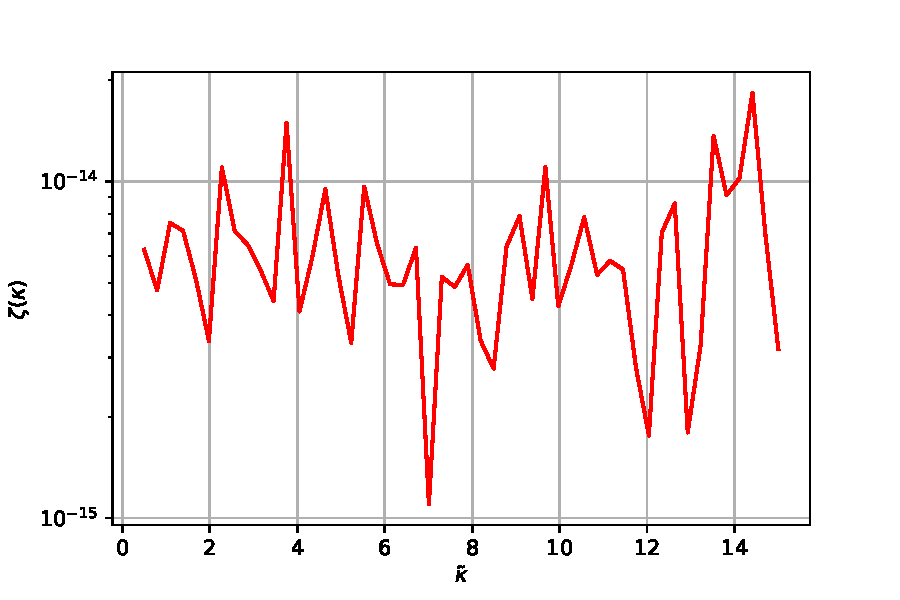
\includegraphics[width=0.5\textwidth]{validate_sol_c_i1,0c_o3,0N_30plotRangeStart_0,5plotRangeEnd_15,0.pdf}
    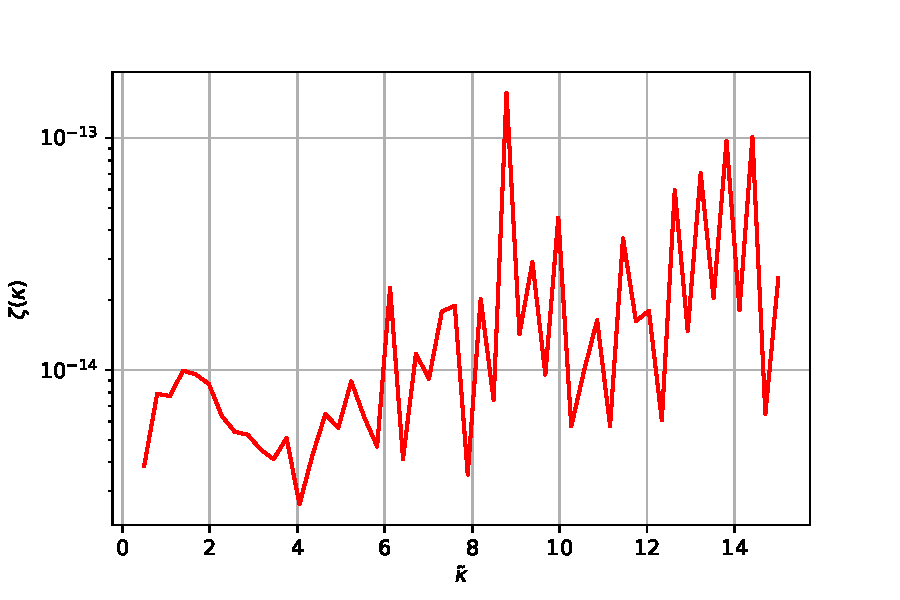
\includegraphics[width=0.5\textwidth]{validate_sol_c_i3,0c_o1,0N_30plotRangeStart_0,5plotRangeEnd_15,0.pdf}
    \caption{Maximum relative residuum of the numerical solution $\zeta$ by wave number. 
    On the left plot we have $c_i = 1, c_o = 3$
    and on the right plot we have $c_i = 3, c_o = 1$. The number of considered Fourier modes was $N = 30$.}
    \label{fig:sol_validation}
\end{figure}
\noindent
As seen in fig. \ref{fig:sol_validation}, the $\zeta$-number is negligible across all values of $\kappa$ and $n$. This validates our derivation of $A_n^{num}$ and $g_n^{num}$.
\subsection{Projector Properties}
\label{subsection:projector_properties}
We validate our matrix $A$ with another method. As mentioned earlier, we must have \(p=0\), if \((U, \theta)\) solves the problem according to \cite{meury2007stable}. 
Assuming $A^{num}_n$ is invertible\footnote{This is fair to assume for most frequencies since the variational problem has a unique solution.}, we can use the remark to validate that our derived matrix $A^{num}_n$ is correct.  We can formulate the property $p = 0$ with regards to $A^{num}_n$. 
Let $V_{\vec{b}} := span( \vec{x}_1, \vec{x}_2)$. 
Then $p = 0$ means that for $\vec{b} \in V_{\vec{b}}$, every solution of  $A_n^{num} \vec{x} = \vec{b}_n$ satisfies $x_3 = 0$. Now let
$P_{V_{\vec{b}}}$ be the projector onto $V_{\vec{b}}$ and $P_3$ be the projector onto $(0, 0, 1)$.
Then $P_3A_n^{-1}P_{V_{\vec{b}}} = 0$. \\
We calculate the euclidian norm of $P_3 (A^{num}_n)^{-1}P_{V_{\vec{b}}}$ for a range of $\kappa$ values to validate this.
\begin{figure}
    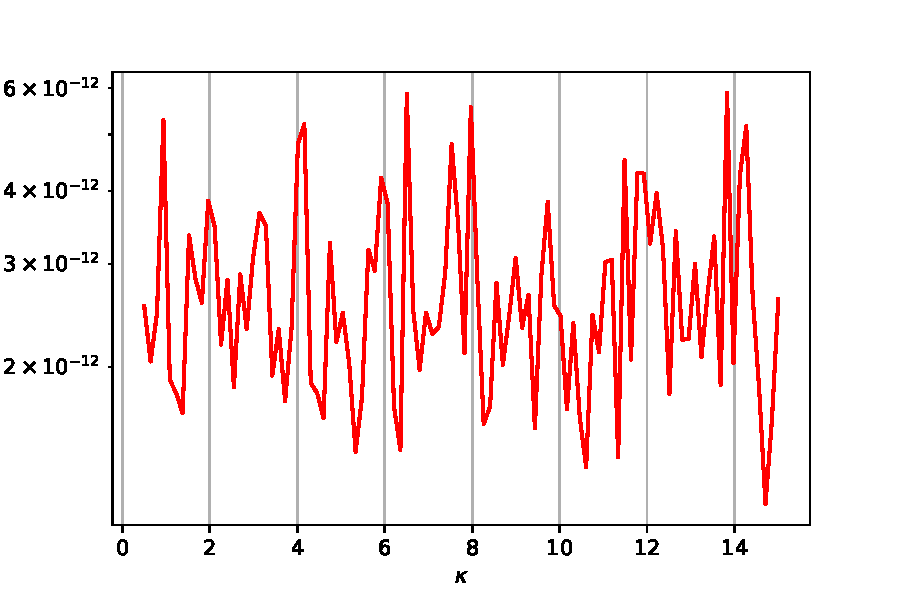
\includegraphics[width=0.5\textwidth]{validate_p_c_i1,0c_o3,0N_100plotRangeStart_0,5plotRangeEnd_15,0.pdf}
    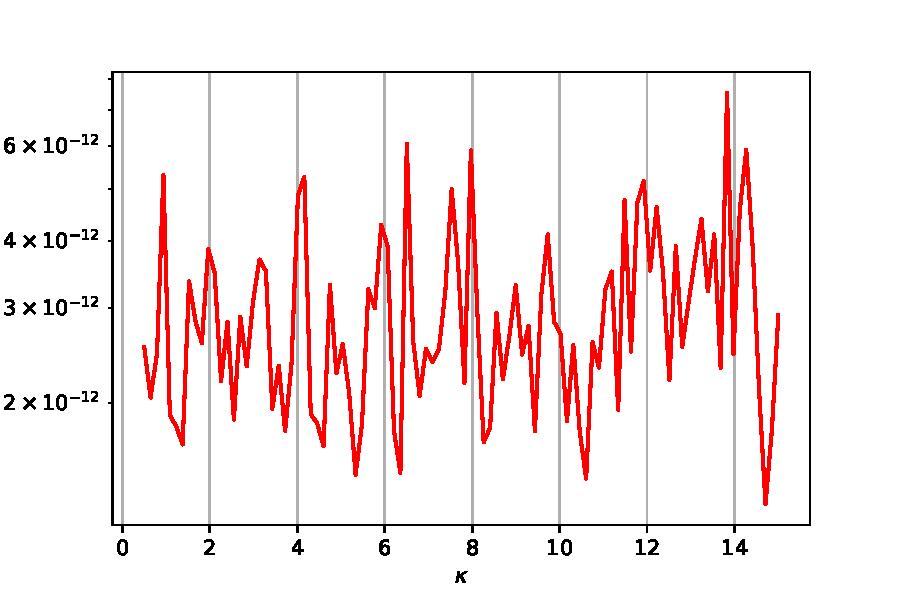
\includegraphics[width=0.5\textwidth]{validate_p_c_i3,0c_o1,0N_100plotRangeStart_0,5plotRangeEnd_15,0.pdf}
    \caption{Euclidian matrix norm of composed matrix  $P_3 (A^{num}_n)^{-1}P_{V_{\vec{b}}}$. 
    On the left plot we have $c_i = 1, c_o = 3$
    and on the right plot we have $c_i = 3, c_o = 1$. The number of considered Fourier modes was $N = 100$.
    }
   \label{fig:p_validation}
\end{figure}
\noindent
Again, as shown in fig. \ref{fig:p_validation}, this is satisfied. This is another validation of our matrix $A_n^{num}$. 



\section{Numerical Results} 
\label{section:numerical_results}
Now, we numerically investigate the operator norm of the inverse operator $A^{-1}$. As established in section \ref{section:spectral_discretisation}, we can compute the inverse of the smallest singular value of $\mathrm{diag}((A_n^{num})_{n = -N}^N)$ for this.
\begin{figure}
    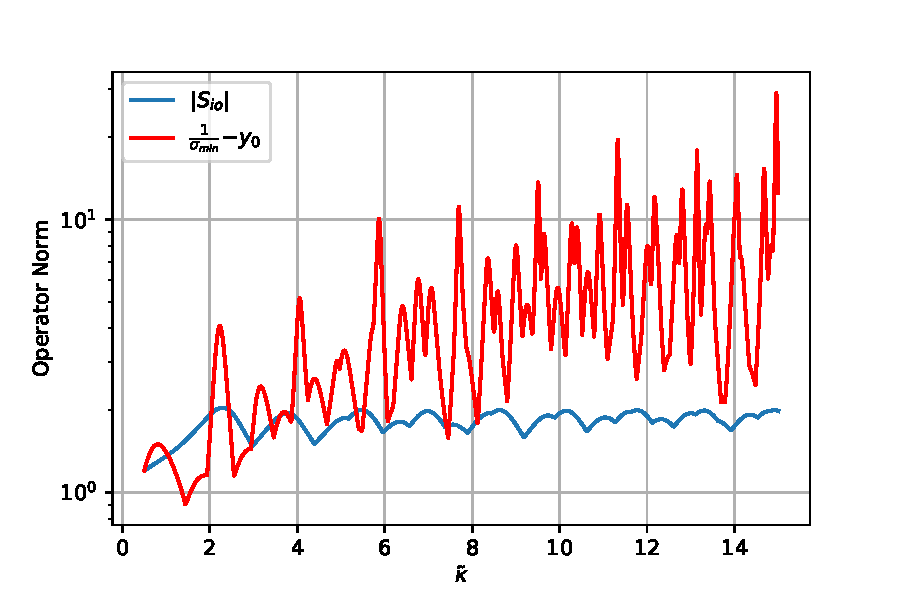
\includegraphics[width=0.5\textwidth]{InvertedMinimumSingularValuec_i1,0c_o3,0N_30eta1,0plotRangeStart_0,5plotRangeEnd_15indexrange_-20,0-0,0_y_0_0,7115197817684848.pdf}
    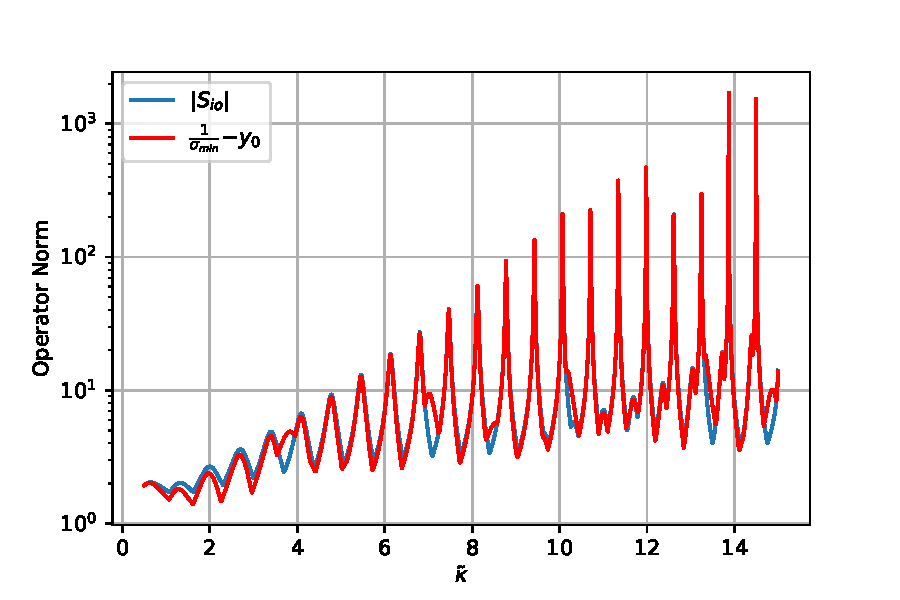
\includegraphics[width=0.5\textwidth]{InvertedMinimumSingularValuec_i3,0c_o1,0N_30eta1,0plotRangeStart_0,5plotRangeEnd_15indexrange_-21,0-0,0_y_0_0,4499662913189779.pdf}
    \caption{Inverted minimum singular value $\left\|A_{\mathcal{S}}^{-1}\right\|_{o p} =\frac{1}{\sigma_{\min }(M)}$of the matrix $M = \mathrm{diag}((A_n^{num})_{n = -N}^N)$ by wave number $\kappa$. Only the first 30 Fourier blocks were considered, as the operator norms were not affected by higher modes. In fact, the highest selected mode was $n = 20$ for the left and $n =21$ for the right plot.
    When plotting the operator norm against $N$ for a fixed $\kappa$, we see that it approaches a constant value for big $N$, justifying the cutoff of $N = 30$. A more detailed explanation is given in the section \nameref{section:appendix}.
    Each of plots is shifted by an absolute value $y_0$ to allow for better comparison with the solution operator.
    In the left plot we have $c_i = 1, c_o = 3$, and $y_0 = 0.712$
    and on the right plot we have $c_i = 3, c_o = 1$, and $y_0 = 0.450$. }
   \label{fig:simulation_results}
\end{figure}
\noindent
The results of the simulation are presented in fig. \ref{fig:simulation_results}  alongside the results for the maximum euclidean norm of the solution operator.\footnote{We picked particular representative cases. More cases are shown in section \ref{section:appendix}.} A derivation of the solution operator is provided in the \nameref{section:appendix}. \\
The solution operator exposes resonance frequencies for the case $c_i = 3, c_o =1$, called  quasi-resonances  in \cite{hiptmair2021spurious}. This resonance behavior is expected physically: If $c_i > c_o$, total internal reflection can undergo. For certain angles of internal reflection, the solution becomes very localised around the boundary $\Gamma$, meaning that the solution operator norm peaks. As we see, peaks in the solution operators coincide with the peaks of the considered inverse boundary integral operator. 
However, in the case $c_i = 1, c_o = 3$ the operator $A^{-1}$ exposes bad condition for some frequencies while the solution operator is regular for all frequencies. This shows that spurious quasi-resonances also occur for the regularised variational formulation. However, it does affect the condition much less than other examples: the STF BIO considered by Hiptmair et al. exposed resonance peaks that were three orders of our magnitude  higher than our considered case \cite{hiptmair2021spurious}. The following proposition helps explain this irregular behavior.

\begin{proposition}
Define
    $\mathcal{L}: \mathcal{H}_{\tilde \kappa}^{\frac{1}{2}} \times \mathcal{H}_{\tilde \kappa}^{-\frac{1}{2}} \rightarrow \mathcal{H}_{\tilde \kappa}^{-\frac{1}{2}} \times \mathcal{H}_{\tilde \kappa}^{\frac{1}{2}} \times \mathcal{H}_{\tilde \kappa}^{-\frac{1}{2}}$ as the map that maps the boundary conditions of eq. \ref{eq:helmholtz} to the right hand side of eq. \ref{eq:operator_formulation}
    $$
        \mathcal{L} = 
        \begin{pmatrix}
            -W_{\kappa} & -id \\
            (K_{\kappa} - \frac{1}{2}) & 0 \\
            W_{\kappa} & 0 \\
        \end{pmatrix}
    $$
and let
 ${E}: \mathcal{H}_{\tilde{\kappa}}^{\frac{1}{2}} \times \mathcal{H}_{\tilde{\kappa}}^{-\frac{1}{2}} \times \mathcal{H}_{\tilde{\kappa}}^{\frac{1}{2}} \rightarrow \mathcal{H}_{\tilde{\kappa}}^{\frac{1}{2}} \times \mathcal{H}_{\tilde{\kappa}}^{-\frac{1}{2}}, {E} = \begin{pmatrix}
    1 & 0 & 0 \\
    0 & 1 & 0 
\end{pmatrix}$.
    Then we can write the solution operator (see definition \ref{def:solution_operator}) as 
    $S = 
    {E}
    A^{-1} \mathcal{L}
    $.
\end{proposition}
\begin{proof}
    Consider the boundary data $f \in \mathcal{H}_{\tilde \kappa}^{\frac{1}{2}} \times \mathcal{H}_{\tilde \kappa}^{-\frac{1}{2}}$. Then by construction we have that the right hand side of eq. \ref{eq:operator_formulation} is $g = \mathcal{L} f$. Applying $A^{-1}$ to the same equation and projecting onto the first two components yields $\begin{pmatrix} U \\ \theta  \end{pmatrix} = {E}A^{-1} \mathcal{L}$. This concludes the proof.
\end{proof}  \noindent
This relationship between $A$ and $S$ implies that the lack of either $E$ or $L$ causes the different resonance behavior between $A$ and $S$. However, it cannot be $E$: analytically, the third solution component $p = 0$ vanishes as mentioned and numerically validated in section \ref{subsection:projector_properties}. Therefore, $L$ must be the origin of the irregularity. To show this, we lift the irregularity by introducing the operator $L_\varepsilon$ for $\varepsilon > 0$: 
\begin{equation} 
\label{eq:L_operator}
L_\varepsilon: \mathcal{H}_{\tilde \kappa}^{-\frac{1}{2}} \times \mathcal{H}_{\tilde \kappa}^{\frac{1}{2}} \times \mathcal{H}_{\tilde \kappa}^{-\frac{1}{2}} \rightarrow \mathcal{H}_{\tilde \kappa}^{-\frac{1}{2}} \times \mathcal{H}_{\tilde \kappa}^{\frac{1}{2}} \times \mathcal{H}_{\tilde \kappa}^{-\frac{1}{2}}, 
L_\varepsilon = 
        \begin{pmatrix}
            -id & -W_{\kappa} &  0\\
            0 & (K_{\kappa} - \frac{1}{2}) & 0 \\
            0 & W_{\kappa} & \varepsilon id \\
        \end{pmatrix}.
\end{equation}
Here we introduced the parameter $\varepsilon$ to formally introduce a new boundary condition parameter, allowing us to invert the operator formally. As this new component is strongly suppressed by $\varepsilon$, it will not impact the outcome. We will use $\varepsilon = 0.01$ in the following calculations. 
Assume that $L_\varepsilon$ is invertible and consider the operator $L_\varepsilon^{-1}A:  \mathcal{H}_{\tilde \kappa}^{-\frac{1}{2}} \times \mathcal{H}_{\tilde \kappa}^{\frac{1}{2}} \times \mathcal{H}_{\tilde \kappa}^{-\frac{1}{2}} \rightarrow  \mathcal{H}_{\tilde \kappa}^{\frac{1}{2}} \times \mathcal{H}_{\tilde \kappa}^{-\frac{1}{2}} \times \mathcal{H}_{\tilde \kappa}^{\frac{1}{2}}$. Note that while we introduced an additional boundary condition parameter in the third argument, it is strongly suppressed by $\varepsilon$. Invertibility is satisfied for the considered case of $\Gamma$, as $L_\varepsilon$ becomes a blockdiagonal operator in the Fourier basis with non-vanishing determinant in each block. 
\begin{figure}
    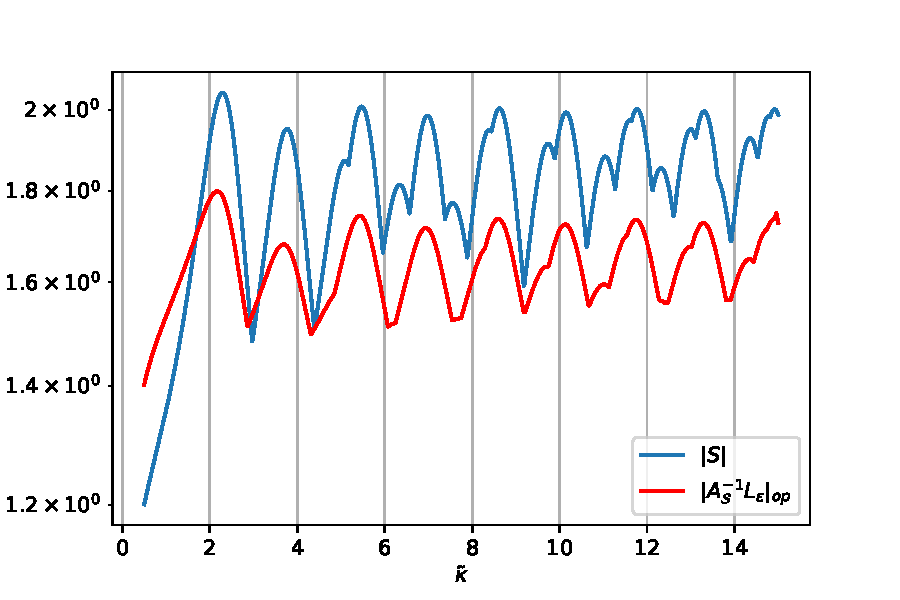
\includegraphics[width=0.5\textwidth]{InvertedMinimumSingularValuec_i1.0c_o3.0N_30eta1.0plotRangeStart_0,5plotRangeEnd_15shiftFirstValue_FalseremoveResonances_Trueindexrange_-15,0-0,0.pdf}
    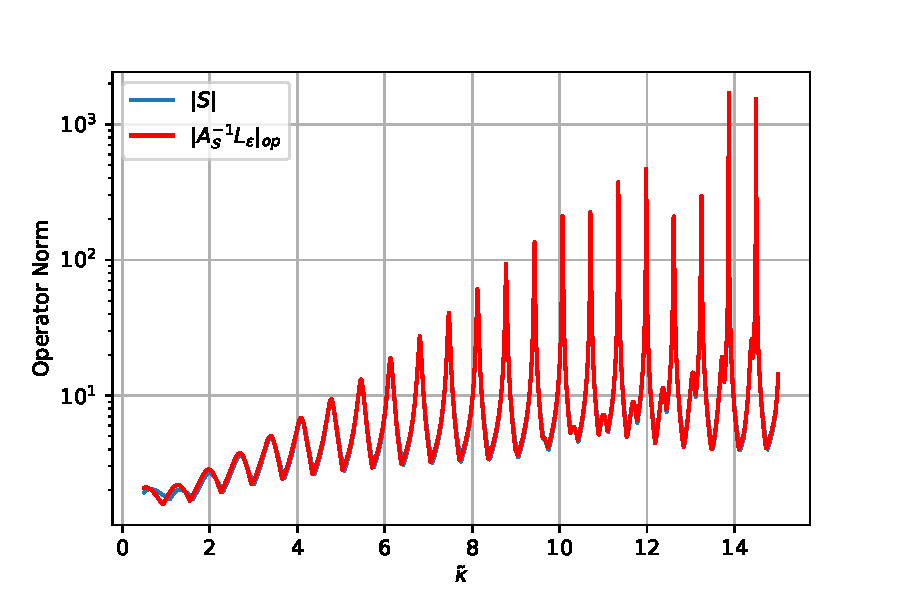
\includegraphics[width=0.5\textwidth]{InvertedMinimumSingularValuec_i3,0c_o1,0N_30eta1,0plotRangeStart_0,5plotRangeEnd_15shiftFirstValue_FalseremoveResonances_Trueindexrange_-22,0-0,0.pdf}
    \caption{Inverted minimum singular value $\left\|A_{\mathcal{S}}^{-1}L_\varepsilon\right\|_{o p} =\frac{1}{\sigma_{\min }(M)}$ by wave number $\kappa$. The highest selected mode out of the considered first $N = 30$ modes was $n = 15$ for the left and $n =22$ for the right plot.
    In the left plot we have $c_i = 1$ and $c_o = 3$
    and on the right plot we have $c_i = 3$ and $c_o = 1$. }
   \label{fig:regularised_results}
\end{figure}
\noindent
As fig. \ref{fig:regularised_results} shows, the irregular resonance  behavior is indeed removed in the case $c_i = 1$, $c_o = 3$ while in the case $c_i = 3$, $c_o = 1$ the resonance behavior still agrees. This implies that the spurious quasi-resonances of the considered regularised formulation operator in eq. \ref{eq:operator_formulation} were indeed caused by the operator applied to the boundary data on the right hand side of the problem.
However, we did not prove the invertibility of $L_\varepsilon$ for general $\Omega^-$. In particular, we did not provide an explicit expression for this inverse.\footnote{While a formal inverse (treating the entries of $L_\varepsilon$ as matrix entries) can be computed symbolically, expressions in the symbolic results may not be well-defined.} Future investigations into this area could include other augmentations of the considered operator that remove these spurious quasi-resonances while also being explicitly expressed for general bounded Lipschitz domains $\Omega^- \subset \mathbb{R}^d$. 


\section{Conclusion}
This report considers a regularised variational formulation of the Helmholtz transmission problem on a two-dimensional disk (eq. \ref{eq:helmholtz}). We converted this variational formulation to an operator formulation (eq. \ref{eq:operator_formulation}) to simplify the  calculations and theoretical results following. After discretizing this formulation (eq. \ref{eq:galerkin_matrix}), we calculated the inverse operator norm of the considered operator $A$ (left side operator of eq. \ref{eq:operator_formulation}) numerically. We found, that for $c_i < c_o$ the operator exposed unphysical spurious quasi-resonances and growth that the solution operator did not (fig. \ref{fig:simulation_results}). However, the occurring resonances, were smaller than for other operator formulations (\cite{hiptmair2021spurious}). By composing with another operator $\mathcal{L}_\varepsilon^{-1}$ (eq. \ref{eq:L_operator}), we were able to remove these spurious quasi-resonances and explain their origin by relating the domain of $A^{-1}$ and the solution operator $S$. However, more general augmentation techniques are required as the considered operator $\mathcal{L}_\varepsilon$ was not proven to be invertible generally, and no explicit inverse was derived for it. 

\section{Appendix}
\label{section:appendix}
\subsection{Numerical Results for other examples}
\begin{figure}
    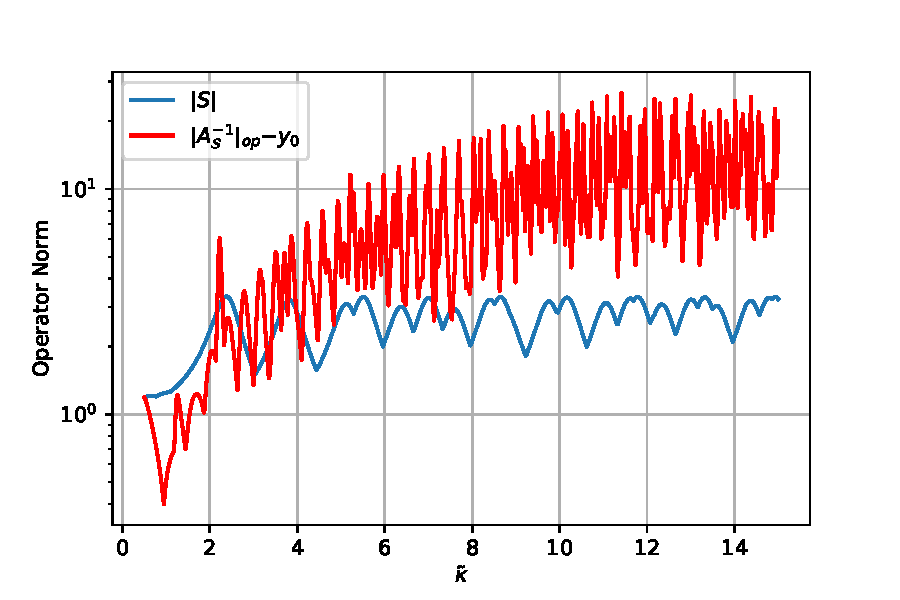
\includegraphics[width=0.5\textwidth]{InvertedMinimumSingularValuec_i1,0c_o10,0N_30eta1,0start_0,5end_15shiftFirstValue_Trueremove_Falseindexrange_-30,0-0,0_y_0_1,3358484167389728.pdf}
    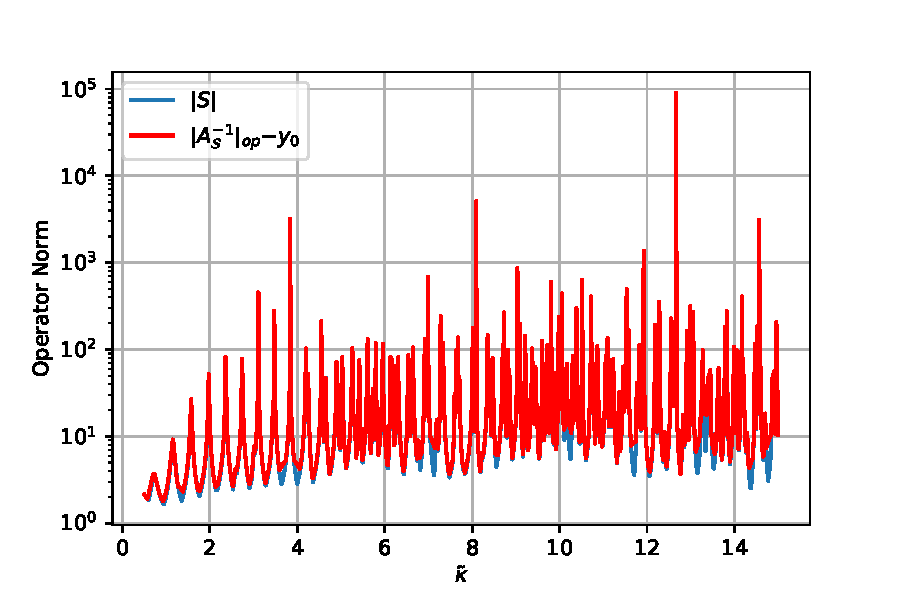
\includegraphics[width=0.5\textwidth]{InvertedMinimumSingularValuec_i10,0c_o1,0N_30eta1,0start_0,5end_15shiftFirstValue_Trueremove_Falseindexrange_-30,0-0,0_y_0_-0,15938792417683234.pdf} 
    \caption{Inverted minimum singular value $\left\|A_{\mathcal{S}}^{-1}\right\|$ by wave number $\kappa$. 
    In the upper left plot we have $c_i = 1$, $c_o = 10$ and $y_0 = 1.336$
    and on the upper right plot we have $c_i = 10$, $c_o = 1$ and $y_0 = -0.159$.}
   \label{fig:c_other_results}
\end{figure}
\noindent
We considered the example $c_i = 1$, $c_o = 3$ and vice versa in section \ref{section:numerical_results}. In fig. \ref{fig:c_other_results} we present other examples for the refractive indices, showing that the overall trends and occurrence of spurious quasi-resonances is very similar to the considered example. \\
\begin{figure}
    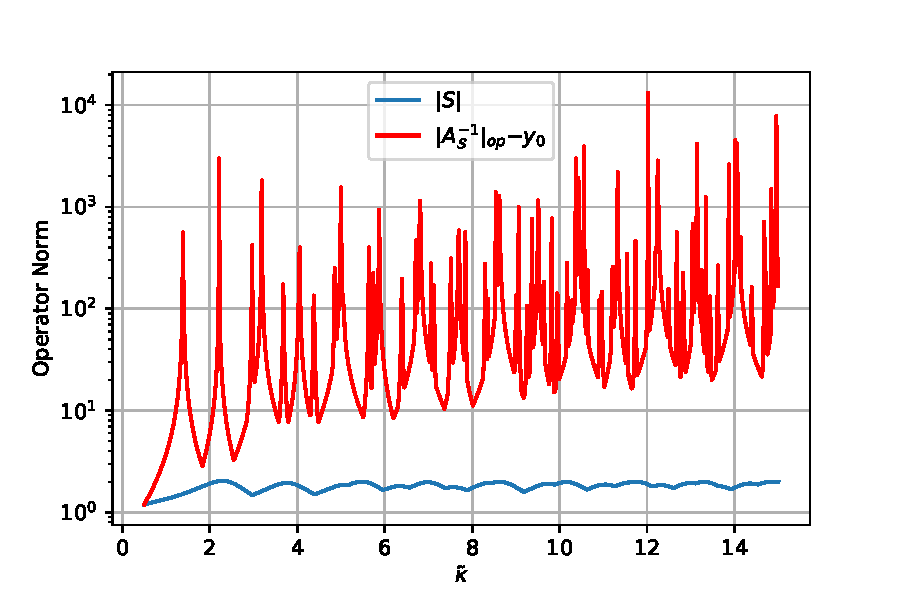
\includegraphics[width=0.5\textwidth]{InvertedMinimumSingularValuec_i1,0c_o3,0N_30eta0start_0,5end_15shiftFirstValue_Trueremove_Falseindexrange_-18,0-0,0_y_0_0,6748762480507995.pdf}
    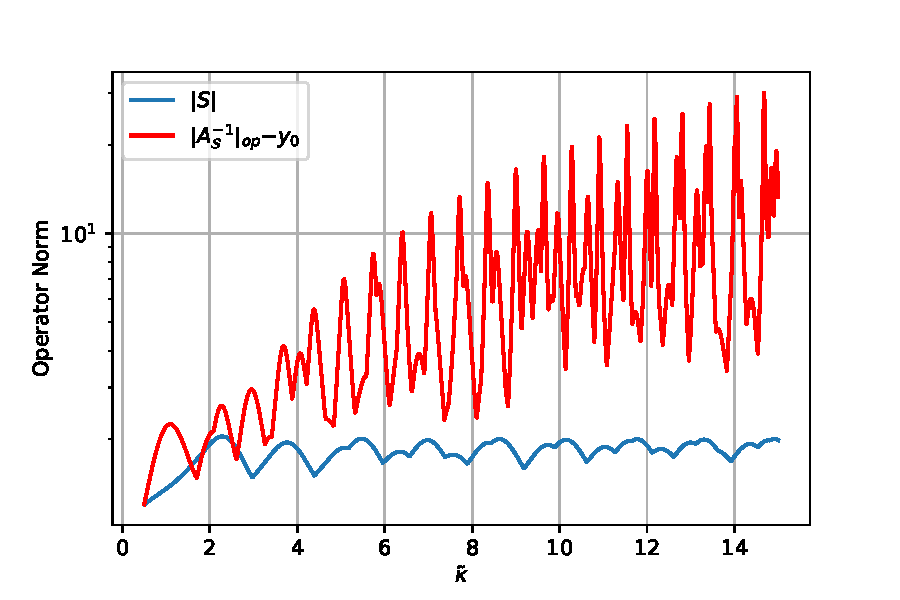
\includegraphics[width=0.5\textwidth]{InvertedMinimumSingularValuec_i1,0c_o3,0N_30eta0,5start_0,5end_15shiftFirstValue_Trueremove_Falseindexrange_-20,0-0,0_y_0_0,6853549487874291.pdf}  \\
    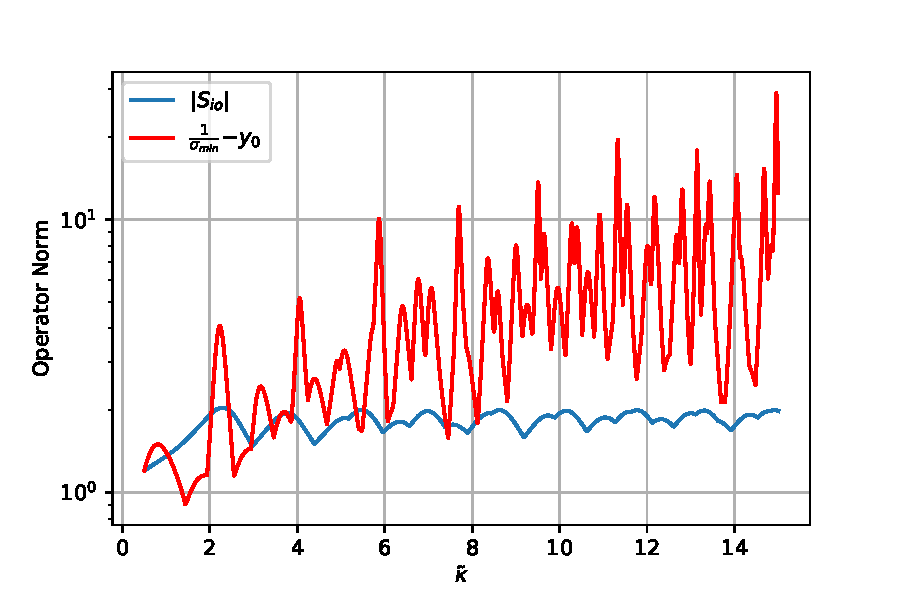
\includegraphics[width=0.5\textwidth]
    {InvertedMinimumSingularValuec_i1,0c_o3,0N_30eta1,0plotRangeStart_0,5plotRangeEnd_15indexrange_-20,0-0,0_y_0_0,7115197817684848.pdf} 
    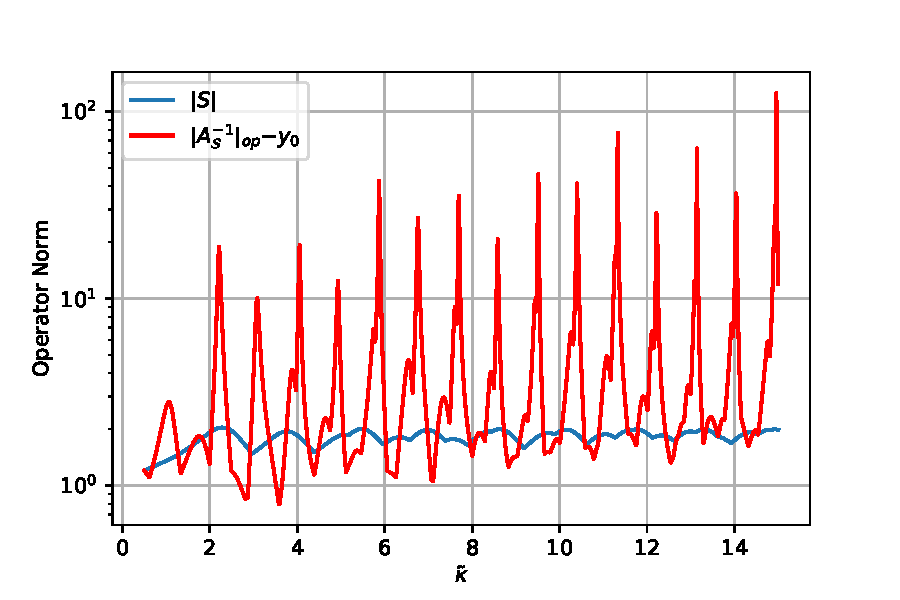
\includegraphics[width=0.5\textwidth]{InvertedMinimumSingularValuec_i1,0c_o3,0N_30eta5,0sart_0,5end_15shiftFirstValue_Trueremove_Falseindexrange_-19,0-0,0_y_0_0,8594171126139554.pdf}  \\
     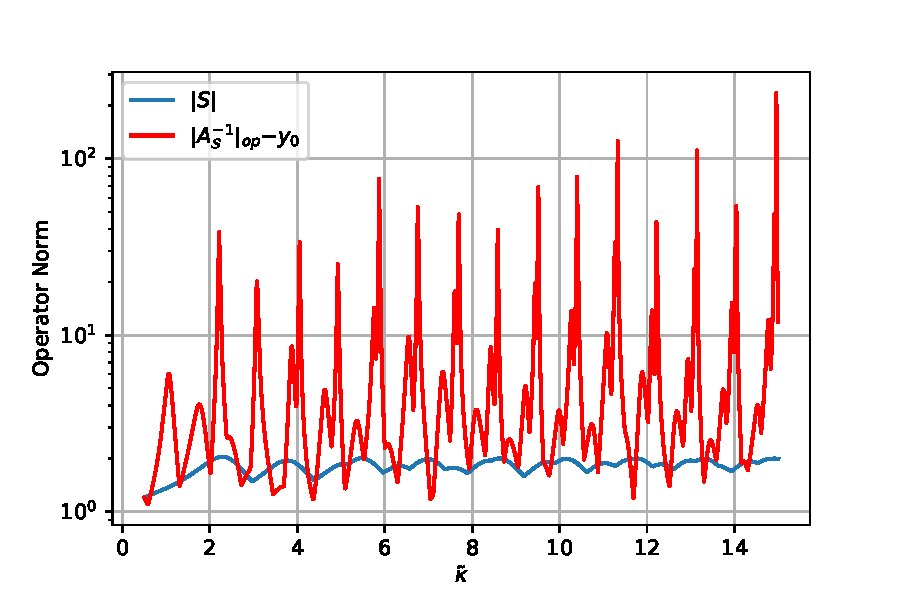
\includegraphics[width=0.5\textwidth]{InvertedMinimumSingularValuec_i1,0c_o3,0N_30eta10start_0,5end_15shiftFirstValue_Trueremove_Falseindexrange_-10,0-0,0_y_0_0,8864570097015256.pdf} 
    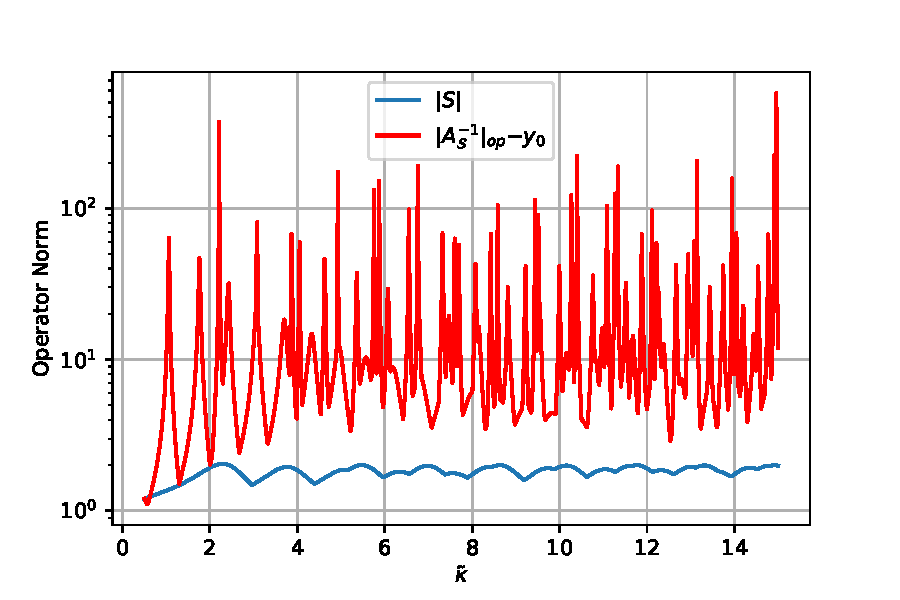
\includegraphics[width=0.5\textwidth]{InvertedMinimumSingularValuec_i1,0c_o3,0N_30eta100,0start_0,5end_15shiftFirstValue_Trueremove_Falseindexrange_-18,0-0,0_y_0_0,8972397818023745.pdf} 
    \caption{Inverted minimum singular value $\left\|A_{\mathcal{S}}^{-1}\right\|$ by wave number $\kappa$. In all six scenarios we have $c_i = 1.0, c_o = 3.0$ and we vary $\eta$. The values of $\eta$ are as follows. Top left: $\eta = 0$, top right: $\eta = 0.5$, middle left: $\eta = 1.0$, middle right: $\eta = 5.0$,  lower left: $\eta = 10.0$, and lower right: $\eta = 100.0$.}
   \label{fig:eta_other_results}
\end{figure}
\noindent
Moreover, we only studied $\eta = 1.0$ in section \ref{section:numerical_results}. As shown in fig. \ref{fig:eta_other_results}, the operator growth is smallest around $\eta = 1.0$ out of the selected values. This is in agreement with the results of P. Meury's doctoral thesis, where he achieved optimal stability around $\eta = 1.0$ \cite{meury2007stable}.
\\
Lastly, we will justify the introduction of a cutoff $N$ for the Fourier modes. In fig. \ref{fig:eta_other_results} the singular value of the operator block $A^{num}_n$ inverse are plotted as a function of the mode $n$. We clearly see, that for $n$ big enough the singular value converges. 
\begin{figure}
\center{
    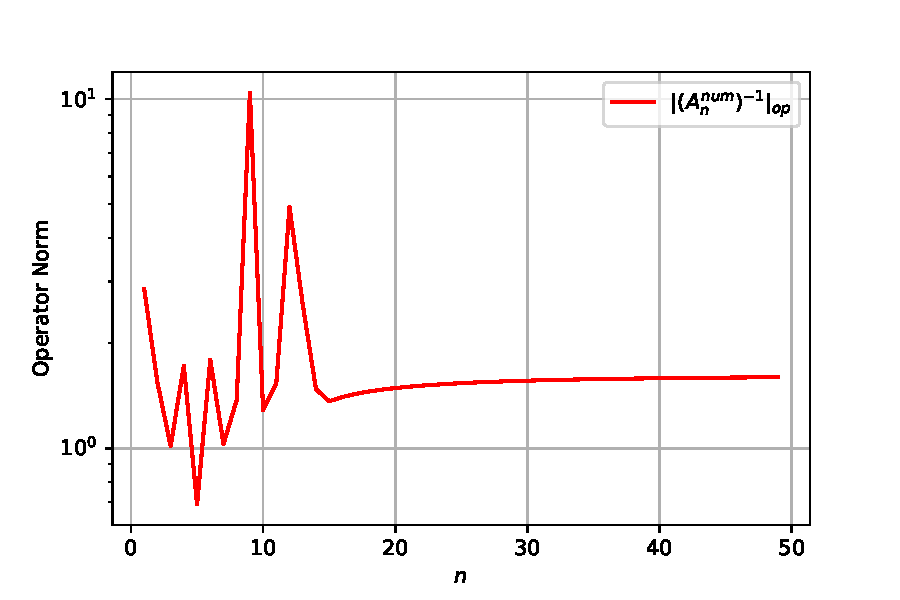
\includegraphics[width=0.5\textwidth]{convergenceTest_c_i1,0c_o_1,0kappa_5,0.pdf}}
    \caption{Inverted singular value $\left\|A^{num}_n\right\|$ for fixed $\kappa$ as a function of the Fourier mode $n$. }
   \label{fig:eta_other_results}
\end{figure}
\noindent
There is also a simple theoretical explanation to justify the cutoff in $n$: consider the matrix $A^{num}_n$ as defined in eq. \ref{eq:galerkin_matrix}. We have the integral representation $J_{n}(x)=\frac{1}{2 \pi i^{n}} \int_{-\pi}^{\pi} e^{i(n \tau-x \sin \tau)} d \tau$ \cite{temme1996special}. 
This directly implies $\alpha_n = O(n)$ as we can switch partial derivative and integral according to the Leibniz integral rule.
Moreover, we know that $\beta_n = O(n^2)$. The following limits can be validated numerically or symbolically:\footnote{Note that the $n$-dependence is not written out explicitly.}
\begin{align}
    \lim\limits_{n \rightarrow \infty} \lambda_n^{(V)} = \frac{1}{2} \nonumber \\
    \lim\limits_{n \rightarrow \infty} \lambda_n^{(K)} = 0 \nonumber \\
    \lim\limits_{n \rightarrow \infty} \frac{\lambda_n^{(W)}}{n} = \frac{1}{2} \nonumber \\
\end{align} and the Bessel and Hankel functions and their derivatives vanish for big enough $n$ and otherwise constant parameters. Therefore, the matrix $A^{num}_n$ behaves the following for big $N$:
$$
    A^{num}_n {\sim} 
    \begin{pmatrix}
        c_\alpha + \frac{1}{2} & - \frac{1}{2} & 0 \\
        \frac{1}{2} & \frac{1}{2} & i \overline{\eta} \\
        - \frac{1}{2} & -\frac{1}{2} & O(n)
    \end{pmatrix} \text { for } n \rightarrow \infty 
$$
where $c_\alpha := \lim\limits_{n\rightarrow \infty} \frac{\alpha_n}{n}$. The smallest singular value of this matrix is given by $\inf\limits_{|x| = 1} \|A^{num}_n x\| $. Since one of the entries in the third column has order $n$, The extremal value of $x$ must have the form $(x^1_n, x^2_n, 0)$. However, the matrix in the first two columns converges, implying convergence of the minimal singular value.

\subsection{Constructing the Solution Operator}
Plugging the Fourier ansatz into eq. \ref{eq:helmholtz} and imposing convergence at the origin and 
the Sommerfeld radiation condition results in
\begin{align}
    u^- = \sum\limits_{n = -\infty}^\infty u_n^- \frac{J_n(\sqrt{ c_i} \tilde \kappa r)}{J_n(\sqrt{ c_i} \tilde \kappa)} e^{i n \phi} \nonumber \\
    u^+ = \sum\limits_{n = -\infty}^\infty u_n^+ \frac{H_n(\sqrt{ c_o} \tilde \kappa r)}{H_n(\sqrt{ c_o} \tilde \kappa)} e^{i n \phi} \nonumber
\end{align}
where $u_n^-$ and $u_n^+$ are the restrictions of $u$ to $\Omega^-$ und $\Omega^+$.\\
Extend $f_i = \sum\limits_{n = -\infty}^\infty f_i^n e^{in\phi}$ for $i=1,2$. The transmission condition $\gamma_{C}^{+} u^{+}=\gamma_{C}^{-} u^{-}+f$ implies 
\begin{align}
    \begin{pmatrix}
        1 & -1 \\
        \sqrt{c_i} \tilde \kappa \frac{J_n^\prime(\sqrt{c_i} \tilde \kappa)}{J_n(\sqrt{c_i} \tilde \kappa)} & 
        -  \sqrt{c_o} \tilde \kappa \frac{H_n^\prime(\sqrt{c_o} \tilde \kappa)}{H_n(\sqrt{c_o} \tilde \kappa)}
    \end{pmatrix} 
    \begin{pmatrix}
        u_n^- \\u_n^+
    \end{pmatrix}
    = 
    \begin{pmatrix}
        f_n^1 \\ f_n^2
    \end{pmatrix}.
\end{align} 
By using the well-known inverse of a 2x2 matrix we obtain 
\begin{equation}
    u_n^- = \zeta(-\sqrt{c_o}\tilde \kappa J_n(\sqrt{c_i} \tilde \kappa) H_n^\prime(\sqrt{c_i} \tilde \kappa)f_n^1 
    + J_n(\sqrt{c_i} \tilde \kappa) H_n(\sqrt{c_o} \tilde \kappa) f_n^2).
\end{equation}
where $\zeta := \frac{1}{\sqrt{c_i} \tilde \kappa J_n^\prime(\sqrt{c_i} \tilde \kappa) H_n(\sqrt{c_o} \tilde \kappa)
-\sqrt{c_o} \tilde \kappa H_n^\prime(\sqrt{c_o}\tilde \kappa) J_n(\sqrt{c_i} \tilde \kappa)
}$.
This presents the solution operator, as we get $\gamma_D^-$ from restriction to the boundary.
$\gamma_N^-$ can be directly obtained by restriction of the normal derivative of $u_n^-$ to the boundary 
which is equivalent to multiplying the Fourier coefficients by $\sqrt{c_i \tilde \kappa}\frac{J_n^\prime(\sqrt{c_i}\tilde \kappa)}{J_n(\sqrt{c_i}\tilde \kappa)}$.
After rescaling the $u_n$, $f_i^n$ to the complete orthonormal system defined in eq. \ref{eq:basis},
we obtain the solution operator matrix: 
\begin{equation}
    S_{io}^n = 
    \zeta
    \begin{pmatrix}
        -\sqrt{c_o}\tilde \kappa J_n(\sqrt{c_i} \tilde \kappa) H_n^\prime(\sqrt{c_i} \tilde \kappa) & 
        \sqrt{n^2 + \tilde \kappa^2} J_n(\sqrt{c_i} \tilde \kappa) H_n(\sqrt{c_o} \tilde \kappa)  \\
        -\frac{1}{\sqrt{n^2 + \tilde \kappa^2}}\sqrt{c_o}\sqrt{c_i} \tilde \kappa^2 J^\prime_n(\sqrt{c_i} \tilde \kappa) H_n^\prime(\sqrt{c_i} \tilde \kappa) & 
        \sqrt{c_i} \tilde \kappa J^\prime_n(\sqrt{c_i} \tilde \kappa) H_n(\sqrt{c_o} \tilde \kappa) \\
    \end{pmatrix}
\end{equation}
\noindent
that maps the Fourier coefficients of $\vec{f}$ in the complete orthonormal system for $\mathcal{H}^{\frac{1}{2}}\times \mathcal{H}^{-\frac{1}{2}}$
 to the Fouier coefficients of $\gamma_C^-u$ in the same basis.

\newpage
\section*{Symbols}

This is an index of symbols repeatedly used in this report with references where the corresponding terms are defined (if applicable).
\begin{itemize}
    \item $H^1(\Omega)$: Sobolev space, \cite{hiptmair2012numerical}.
    \item $H_{\mathrm{loc}}^{1}\left(\Omega^{\pm}\right)$:  \(H_{\text {loc }}^{1}\left(\Omega^{\pm}, \Delta\right):=\left\{v: \chi v \in H^{1}\left(\Omega^{\pm}\right), \Delta(\chi v) \in L^{2}\left(\Omega^{\pm}\right)\right.\)for all \(\left.\chi \in C_{\text {comp }}^{\infty}\left(\mathbb{R}^{d}\right)\right\}\), section \ref{section:introduction}
    \item $H^{\frac{1}{2}}(\Gamma)$: Dirichlet trace space, \cite{hiptmair2018advanced}.
    \item $H^{-\frac{1}{2}}(\Gamma)$: Neumann trace space, \cite{hiptmair2018advanced}.
    \item $\Omega^{-}$: Generally a bounded Lipschitz domain.  $\Omega^{0} = B_1(0) \subset \mathbb{R}^2$ for most of the report, section \ref{section:introduction}. 
    \item $\Omega^{+}$: \(\Omega^{+}:=\mathbb{R}^{d} \backslash \overline{\Omega^{-}}\), section \ref{section:introduction}.
    \item $\Gamma$: \(\Gamma:=\partial \Omega^{-}=\partial \Omega^{+}\).
    \item \(\operatorname{grad}_{\Gamma}\): surface gradient, \cite{sauter2010boundary}.
    \item \(\operatorname{grad}_{\Gamma}\): adjoint map of $\hat{\phi} \operatorname{grad}_{\Gamma}$, \ref{section:operator_formulation}.
    \item $\varphi^{\pm}$: \(\varphi^{\pm}:=\left.\varphi\right|_{\Omega^{\pm}}\), section \ref{section:introduction}.
    \item $C_{\text {comp }}^{\infty}\left(\mathbb{R}^{d}\right)$: Smooth functions with compact support
    \item $\gamma_{D}^{\pm}$: Dirichlet trace operators, section \ref{section:introduction}.
    \item $\gamma_{N}^{\pm}$: Neumann trace operator, section \ref{section:introduction}.
    \item \(\gamma_{C}^{\pm}\): Cauchy trace, section \ref{section:introduction}.
    \item $f$: Boundary conditions of Helmholtz transmission problem, section \ref{section:introduction}.
    \item $\kappa, \tilde \kappa$: Wave number, section \ref{section:introduction}.
    \item $c_i, c_o, \tilde c$: Refractive indices, section \ref{section:introduction}.
    \item $U, \theta, p$: Solution of Helmholtz transmission problem, section \ref{section:introduction} \& section \ref{section:regularized_variational_formulation}.
    \item $S$: Solution operator, section \ref{section:introduction}.
    \item $\mathrm{DtN}^-_\kappa$: Interior Dirichlet-to-Neumann map, section \ref{section:definitions}.
    \item $\mathrm{V}_\kappa, \mathrm{K}_\kappa, \mathrm{K}^\prime_\kappa, \mathrm{W}_\kappa$: Boundary integral operators, section \ref{section:definitions}.
    \item $q_\kappa(\cdot, \cdot), b(\cdot, \cdot)$: Bilinear forms in regularized variational formulation, section \ref{section:regularized_variational_formulation}.
    \item $g_i$: Right hand side of regularized variational formulation, section \ref{section:regularized_variational_formulation}.
    \item \(\mathcal{H}^{s}(\Gamma)_{\tilde \kappa}\): Fourier Sobolev Hilbert space, section \ref{section:operator_formulation}.
    \item $A$: Left hand side operator in the regularized operator formulation, section \ref{section:operator_formulation}.
    \item $\mathcal{B}$: Right hand side boundary value operator in the regularized operator formulation, section \ref{section:operator_formulation}.
    \item $\mathcal{S}^s_N$: Restricted Sobolev space for numerical calculations, section \ref{section:spectral_discretisation}.
    \item $\lambda^{(\mathrm{V})}, \lambda^{(\mathrm{K})}, \lambda^{(\mathrm{K}^\prime)}, \lambda^{(\mathrm{W})}$: Fourier eigenvalues of boundary value operators, section \ref{section:spectral_discretisation}.
    \item $\alpha_n, \beta_n$: Fourier eigenvalues of operators occurring in regularised operator, section \ref{section:spectral_discretisation}.
    \item $A^{num}_n$: Galerkin matrix, section \ref{section:spectral_discretisation}.
    \item \(\mathcal{L}_\varepsilon\): augmenting operator  for  $A$, section \ref{section:numerical_results}.
\end{itemize}
    
    

\section*{Code}
Calculations and plots were implemented in Python. The corresponding files are available \href{https://github.com/FredericJorgensen/spurious-quasi-resonances-coupled-variational-formulation}{here}.

\bibliography{references}
\bibliographystyle{ieeetr}

\end{document}
